\RequirePackage{fix-cm}
\documentclass[smallextended,final]{svjour3}  % onecolumn (second format)
\smartqed  % flush right qed marks, e.g. at end of proof

% Insert here the call for the packages your document requires
\usepackage{graphicx}
\usepackage{tikz}     % For adding axes to plots
\usetikzlibrary{positioning}
\usepackage{graphicx} % For including PDFs
\usepackage{amsmath}  % assumes amsmath package installed
\usepackage{amssymb}  % assumes amsmath package installed
\usepackage{booktabs} % For formal tables
\usepackage{tabularx} % For tables with nice column widths.
\usepackage[colorlinks,allcolors=blue]{hyperref}
\usepackage{float}    % For controlling the placement of tables.

%
% please place your own definitions here and don't use \def but
% \newcommand{}{}

%% Command for creating multiplie-line cells inside a table environment
\newcommand{\multilinecell}[2][c]{%
  \begin{tabular}[#1]{@{}c@{}}#2\end{tabular}}

\newcolumntype{d}[1]{D{.}{.}{#1}}

%% Create a ``Lemma'' environment that does not have italics font.
\spnewtheorem{plainlemma}{Lemma}{\bf}{}
%% Create a ``Theorem'' environment that is not numbered.
\spnewtheorem*{onetheorem}{Theorem}{\bf}{}
%% Create a ``Proof'' environment that starts with 'Proof.'
\spnewtheorem*{proofdot}{Proof.}{\it}{}

%% \newcommand{\Bigl}{\mathopen\Big}
%% \newcommand{\Bigr}{\mathclose\Big}
%
% Insert the name of "your journal" with
\journalname{Numerical Algorithms}
%
\begin{document}

\title{Interpolation of Sparse High-Dimensional Data\thanks
  {This work was supported by the National Science Foundation Grant CNS-1565314.}
}
% \subtitle{Do you have a subtitle?\\ If so, write it here}
%\titlerunning{Short form of title}        % if too long for running head

\author{Thomas C. H. Lux   \and
  Layne T. Watson          \and
  Tyler H. Chang           \and
  Yili Hong                \and
  Kirk Cameron
}

%\authorrunning{Short form of author list} % if too long for running head

\institute{Thomas Lux \at
  Virginia Polytechnic Institute \& State University (VPI\&SU) \\
  Blacksburg, VA 24061 \\
  \email{tchlux@vt.edu}
}

\date{Received: date / Accepted: date}
% The correct dates will be entered by the editor

\maketitle

\begin{abstract}
Increases in the quantity of available data have allowed all fields of
science to generate more accurate models of multivariate phenomena.
Regression and interpolation become challenging when the dimension of
data is large, especially while maintaining tractable computational
complexity. Regression is a popular approach to solving approximation
problems with high dimension, however there are often advantages to
interpolation. This paper presents a novel and insightful error bound
for (piecewise) linear interpolation in arbitrary dimension and
contrasts the performance of some interpolation techniques with
popular regression techniques. Empirical results demonstrate the
viability of interpolation for moderately high dimensional
approximation problems, and encourage broader application of
interpolants to multivariate approximation in science.

\keywords{approximation \and regression \and interpolation \and high
  dimension \and error bound}
% \PACS{PACS code1 \and PACS code2 \and more}
% \subclass{MSC code1 \and MSC code2 \and more}
\end{abstract}

%     Introduction     
%======================

%% ===================================================================
\section{Introduction}
\label{sec:introduction}

Regression and interpolation are problems of considerable importance
that find applications across many fields of science. Pollution and
air quality analysis \cite{de2008field}, energy consumption management
\cite{lazos2014optimisation}, and student performance prediction
\cite{cortez2008using,lux2016applications} are a few of many
interdisciplinary applications of multivariate regression for
predictive analysis. As discussed later, these techniques can also be
applied to prediction problems related to forest fire risk assessment
\cite{cortez2007data}, Parkinson's patient clinical evaluations
\cite{tsanas2010accurate}, local rainfall and weather
\cite{williams2009rattle}, credit card transactions
\cite{pozzolo2015calibrating}, and high performance computing (HPC)
file input/output (I/O) \cite{lux2018nonparametric}.

Regression and interpolation have a considerable theoretical base in
one dimension \cite{cheney2009course}. Splines in particular are well
understood as an interpolation technique in one dimension
\cite{de1978practical}, particularly B-splines. Tensor products of
B-splines \cite{unther1996interpolating} or other basis functions have
an unfortunate exponential scaling with increasing
dimension. Exponential scaling prohibits tensor products from being
reasonably applied beyond three-dimensional data. In order to address
this dimensional scaling challenge, C. de Boor and others proposed box
splines \cite{de2013box}, of which one of the approximation techniques
in this work is composed \cite{lux2018novel}.

The theoretical foundation of low dimensional interpolation allows the
construction of strong error bounds that are absent from high
dimensional problems. This work extends some known results regarding
the secant method \cite{dennis1996numerical} to construct an
interpolation error bound for problems of arbitrary dimension. These
error bounds are useful, considering the same cannot be said for
regression algorithms in general. The maximum complexity of an
interpolant is bounded by the amount of data available, while the
maximum complexity of a regressor is bounded by both the amount of
data and the chosen parametric form. For this reason, generic uniform
bounds are largely unobtainable for regression techniques on arbitrary
approximation problems, even when the approximation domain is bounded.

Aside from theoretical motivation for the use of interpolants, there
are often computational advantages as well. Interpolants do not have
the need for \textit{fitting} data, or minimizing error with respect
to model parameters. In applications where the amount of data is large
and the relative number of predictions that need to be made for a
given collection of data is small, the direct application of an
interpolant is much less computationally expensive.

In this work, multivariate interpolation is defined given a closed
convex subset $Y$ of a metrizable topological vector space with metric
$s$, some function $f:\mathbb{R}^d \rightarrow Y$ and a set of points
$X = \bigl\{x^{(1)}$, $\ldots$, $x^{(n)}\bigr\} \subset \mathbb{R}^d$,
along with associated function values $f\bigl(x^{(i)}\bigr)$. The goal
is to construct an approximation $\hat f: \mathbb{R}^d \rightarrow Y$
such that $\hat f\bigl(x^{(i)}\bigr) = f\bigl(x^{(i)}\bigr)$ for all
$i = 1$, $\ldots$, $n$. It is often the case that the form of the true
underlying function $f$ is unknown, however it is still desirable to
construct an approximation $\hat f$ with small approximation error at
$y \notin X$. The two metric spaces that will be discussed in this
work are the real numbers with metric $s(x,y) = |x-y|$, and the set of
cumulative distribution functions (CDFs) with the Kolmogorov-Smirnov
(KS) statistic \cite{lilliefors1967kolmogorov} as a metric.

Multivariate regression is often used when the underlying function is
presumed to be stochastic, or stochastic error is introduced in the
evaluation of $f$. Hence, multivariate regression relaxes the
conditions of interpolation by choosing parameters $P$ defining $\hat
f(x;P)$ to minimize the error vector $\Bigl( \bigl | \hat f
\bigl(x^{(1)};P\bigr) - f\bigl(x^{(1)}\bigr) \bigr|$, $\ldots$, $\bigl
| \hat f \bigl(x^{(n)}; P\bigr) - f\bigl(x^{(n)}\bigr) \bigr | \Bigr)$
in some norm. The difficult question in the case of regression is
often what parametric form to adopt for any given application.

The most challenging problem when scaling in dimension is that the
number of possible interactions between dimensions grows
exponentially. Quantifying all possible interactions becomes
intractable, and hence beyond three-dimensional data mostly linear
models are used. That is not to say nonlinear models are absent, but
nonlinearities are often either preconceived or model pairwise
interactions between dimensions at most. Even globally nonlinear
approximations such as neural networks are constructed from
compositions of summed low-interaction functions
\cite{clevert2015fast}.

Provided the theoretical and practical motivations for exploring
interpolants, the main objective of this work is to study the
empirical performance differences in both accuracy and computational
expense between a set of interpolation techniques and a set of common
regression techniques. The main contributions of this work are a sharp
theoretical error bound for (piecewise) linear interpolation in
arbitrary dimension and multiple empirical comparisons that illustrate
potential advantages of interpolation.

The remainder of this paper is organized as follows. Sections
\ref{sec:regression} and \ref{sec:interpolation} present the
multivariate models. Section \ref{sec:error} gives the error measuring
methodology that is used for collecting empirical results. Section
\ref{sec:theory} contains the theoretical error bounds for
interpolation as well as an analytic test for demonstration. Section
\ref{sec:data} presents the data sets for empirical approximation
analysis and the approximation results for all models on these data
sets. Section \ref{sec:discussion} analyzes and discusses the results,
their implications, and their limitations. Finally, Section
\ref{sec:conclusion} concludes.

%% ===================================================================
\section{Multivariate Regression}
\label{sec:regression}
Multivariate regressors are capable of accurately modeling a complex
dependence of a response (in $Y$) on multiple variables (represented
as a points in $\mathbb{R}^{d}$). The approximations to some (unknown)
underlying function $f: \mathbb{R}^d \rightarrow Y$ are chosen to
minimize some error measure related to data samples
$f\bigl(x^{(i)}\bigr)$. For example, least squares regression uses the
sum of squared differences between modeled function values and true
function values as an error measure. In this section and the next,
some techniques are limited to approximating real valued functions ($Y
\subset \mathbb{R}$). These techniques can be extended to real
vector-valued ranges by repeating the construction for each component
of the vector output. Throughout the following, $x$ denotes a
$d$-tuple, $x_i$ the $i$th component of $x$, and $x^{(i)}$ the $i$th
$d$-tuple data point. Different symbols are used to represent the
approximation function $\hat f$.

\subsection{Multivariate Adaptive Regression Splines}
\label{sec:mars}
This approximation was introduced in \cite{friedman1991multivariate}
and subsequently improved to its current version in
\cite{stanford1993fast}, called fast multivariate adaptive regression
splines (Fast MARS). In Fast MARS, a least squares fit model is
iteratively built by beginning with a single constant valued function
and adding two new basis functions at each iteration of the form
\begin{align*}
  B_{2j-1}(x) &= B_l(x) \bigl(x_i-x^{(p)}_i\bigr)_+, \\
  B_{2j}(x) &= B_k(x) \bigl(x_i-x^{(p)}_i\bigr)_- ,
\end{align*}
where $j$ is the iteration number, $1 \le p \le n$, and $B_l(x)$,
$B_k(x)$ are basis functions from the previous iteration,
 $$w_+ = \begin{cases} w, & w \geq 0 \\ 0, & w < 0 \end{cases},$$
and $w_- = (-w)_+$. After iteratively constructing a model, MARS then
iteratively removes basis functions that do not contribute to goodness
of fit. In effect, MARS creates a locally component-wise tensor
product approximation of the data. The overall computational
complexity of Fast MARS is $\mathcal{O}(n d m^3)$ where $m$ is the
maximum number of underlying basis functions. This paper uses an
implementation of Fast MARS \cite{rudy2017pyearth} with $m = 200$
throughout all experiments.

\subsection{Support Vector Regressor}
\label{sec:svr}
Support vector machines are a common method used in machine learning
classification tasks that can be adapted for the purpose of regression
\cite{basak2007support}. How to build a support vector regressor (SVR)
is beyond the scope of this summary, but the resulting functional fit
$p : \mathbb{R}^d \rightarrow \mathbb{R}$ has the form
 $$ p(x)  = \sum_{i=1}^{n}a_i K\bigl(x,x^{(i)}\bigr) + b ,$$
where $K$ is the selected kernel function, $a_i \in \mathbb{R}^n$, 
$b \in \mathbb{R}$ are coefficients to be solved for simultaneously.
The computational complexity of the SVR is $\mathcal{O}(n^2dm)$, with
$m$ being determined by the minimization convergence criterion. This
paper uses the scikit-learn SVR \cite{scikit-learn} with a radial
basis function kernel.

\subsection{Multilayer Perceptron Regressor}
\label{sec:mlp}
The neural network is a well studied and widely used method for both
regression and classification tasks
\cite{hornik1989multilayer,rumelhart1988learning}. When using the
rectified linear unit (ReLU) activation function
\cite{dahl2013improving} and fitting the model with stochastic
gradient descent (SGD) or BFGS minimization techniques
\cite{goh2017why,moller1993scaled,robbins1951stochastic}, the model
built by a multilayer perceptron uses layers $l : \mathbb{R}^{i}
\rightarrow \mathbb{R}^{j}$ defined by
 $$ l(u) = \bigl( u^t W_l + c_l \bigr)_+ ,$$
where $c_l \in \mathbb{R}^j$ and $W_l$ is the $i \times j$ weight
matrix for layer $l$. In this form, the multilayer perceptron (MLP)
produces a piecewise linear model of the input data. The computational
complexity of training a multilayer perceptron is $\mathcal{O}(n d
m)$, where $m$ is determined by the sizes of the layers of the network
and the stopping criterion of the minimization used for finding
weights. This paper uses an MLP built from Keras and Tensorflow to
perform regression \cite{tensorflow2015-whitepaper,chollet2015keras}
with ten hidden layers each having thirty two nodes (a total of
approximately ten thousand parameters), ReLU activation, and five
thousand epochs of SGD for training.

%% ===================================================================
\section{Multivariate Interpolation}
\label{sec:interpolation}
The following interpolation techniques demonstrate a reasonable
variety of approaches to interpolation. All of the presented
interpolants produce approximations that are continuous in value,
which is often a desirable property in applied approximation problems.

\subsection{Delaunay}
\label{sec:delaunay}

The Delaunay triangulation is a well-studied geometric technique for
producing an interpolant \cite{lee1980two}. The Delaunay triangulation
of a set of data points into simplices is such that there are no data
points inside the sphere defined by the vertices of each simplex. For
a $d$-simplex S with vertices $x^{(0)}$, $x^{(1)}$, $\ldots$,
$x^{(d)}$, and function values $f\bigl(x^{(i)}\bigr)$, $i=0$,
$\ldots$, $d$, $y \in S$ is a unique convex combination of the
vertices,
 $$ y = \sum_{i=0}^{d} w_i x^{(i)}, \quad \sum_{i=0}^{d} w_i = 1, \quad w_i \geq 0, \quad i=0,\ldots,d, $$
and the Delaunay interpolant $\hat f(y)$ at $y$ is given by
 $$ \hat f(y) = \sum_{i=0}^{d} w_i f\bigl(x^{(i)}\bigr). $$ The
computational complexity of Delaunay interpolation (for the
implementation used \cite{chang2018polynomial}) is $\mathcal{O}(k n
d^3)$. Given pathological data the entire triangulation could be
computed with $k = n^{\lceil d / 2 \rceil}$, but the average case yields
$k = d \log d$ and is capable of scaling reasonably to $d \leq 50$. In
the present application, a Delaunay simplex $S$ containing $y$ is
found, then the $d+1$ vertices (points in $X$) of $S$ are used to
assign weights to each vertex and produce the predicted function value
for point $y$.

\subsection{Modified Shepard}
\label{sec:modified-shepard}

The modified Shepard method used here (ShepMod) generates a continuous
approximation based on Euclidean distance and resembles a nearest
neighbor interpolant \cite{cover1967nearest}. This model is a type of
\textit{metric interpolation}, also called a Shepard method
\cite{gordon1978shepard,shepard1968two}. The interpolant has the form
 $$ p(x) = \frac{\sum\limits_{k=1}^{n}W_k(x)f\bigl(x^{(k)}\bigr)}
     {\sum\limits_{k=1}^{n}W_k(x)} ,$$
where $W_k(x) = \bigl(r_k - \bigl\|x - x^{(k)}\bigr\|\bigr)_+^2 \big/
\bigl\|x - x^{(k)}\bigr\|_2^2$ and $r_k \in \mathbb{R}$ is the
smallest radius such that at least $d+1$ other points $x^{(j)}$, $j
\not = k$, are inside the closed Euclidean ball of radius $r_k$ about
$x^{(k)}$. The computational complexity of ShepMod is
$\mathcal{O}(n^2d)$. This paper uses a Fortran 95 implementation of
ShepMod derived from SHEPPACK \cite{thacker2010algorithm}.

\subsection{Linear Shepard}
The linear Shepard method (LSHEP) is a blending function using local
linear interpolants, a special case of the general Shepard algorithm
\cite{thacker2010algorithm}. The interpolant has the form
 $$ p(x) = \frac{\sum\limits_{k=1}^{n}W_k(x)P_k(x)}
 {\sum\limits_{k=1}^{n}W_k(x)} ,$$
where $W_k(x)$ is a locally supported weighting function and $P_k(x)$
is a local linear approximation to the data satisfying
$P_k\bigl(x^{(k)}\bigr) = f\bigl(x^{(x)}\bigr)$. The computational
complexity of LSHEP is $\mathcal{O}(n^2d^3)$. This paper uses the
Fortran 95 implementation of LSHEP in SHEPPACK
\cite{thacker2010algorithm}.

\subsection{Box Splines}
\label{sec:box-splines}

The box spline model used here is a sparse grid interpolation
technique built from overlapping box splines \cite{de2013box}. The box
splines serve as basis functions that are shifted and scaled to have
support over box shaped regions. The boxes are constructed in a way to
guarantee a covering of the domain \cite{lux2018novel}. Given a set of
box splines $\bigl\{b^{x^{(i)}}\bigr\}$ with the iterative box
properties outlined in \cite{lux2018novel} and anchored at interior
points $\bigl\{x^{(i)}\bigr\}$,
 $$ \hat f(y) = \frac{\sum\limits_{i=1}^n b^{x^{(i)}}(y) f\bigl(x^{(i)}\bigr)}{\sum\limits_{i=1}^n b^{x^{(i)}}(y)}. $$
Note that the box splines always satisfy
$b^{x^{(i)}}\bigl(x^{(j)}\bigr) = \delta_{ij}$ and $b^{x^{(i)}}(y)
\geq 0$. The computational complexity of interpolation via the box
spline model is $\mathcal{O}(n^2 d)$.

\subsection{Voronoi}
\label{sec:voronoi}

The nearest neighbor algorithm \cite{cover1967nearest} is a
well-studied technique for classification and approximation. Nearest
neighbor inherently utilizes the convex region $C^{x^{(i)}}$ (Voronoi
cell \cite{dirichlet1850reduction}) consisting of all points closer to
$x^{(i)}$ than to any other point $x^{(j)}$. The Voronoi model smooths
the nearest neighbor approximation by utilizing the Voronoi cells to
define support via a generic basis function $v: \mathbb{R}^d
\rightarrow \mathbb{R}_+$ given by
 $$ v^{x^{(i)}}(y) = \left(1 - \frac{\bigl\|y - x^{(i)}\bigr\|_2}
 {2 \ h \bigl(y - x^{(i)} \mid x^{(i)}\bigr)} \right)_+, $$
where $h\bigl(w \mid x^{(i)}\bigr)$ is the distance between $x^{(i)}$
and the boundary of the Voronoi cell $C^{x^{(i)}}$ in the direction
$w$. $v^{x^{(i)}}\bigl(x^{(j)}\bigr) = \delta_{ij}$ and $v^{x^{(i)}}$
has local support, giving the interpolated value
 $$ f(y) = \frac{\sum\limits_{i=1}^n v^{x^{(i)}}(y)
  f\bigl(x^{(i)}\bigr)}{\sum\limits_{i=1}^n v^{x^{(i)}}(y)}, $$
where $0 \leq v^{x^{(i)}}(y) \leq 1$. The computational complexity of
interpolation via this Voronoi model is $\mathcal{O}(n^2 d)$. All of
the approximations are an interpolant involving a convex combination
of known function values $f\bigl(x^{(i)}\bigr)$.

%% ===================================================================
\section{Measuring Error}
\label{sec:error}

\begin{figure}[htb]
  \centering
  \begin{tikzpicture}
    \node (img)  {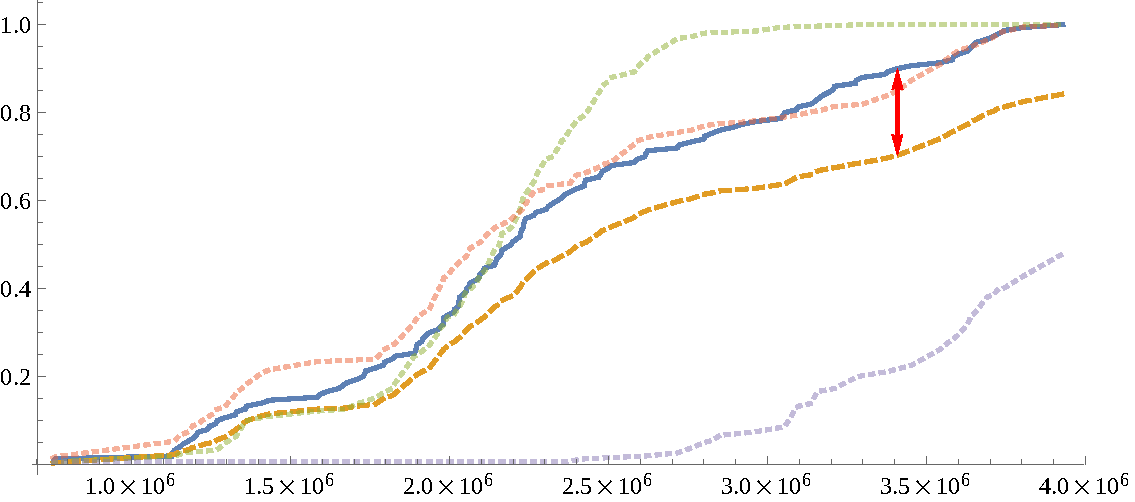
\includegraphics[width=0.75\textwidth,]{Fig1.pdf}};
    \node[below=of img, node distance=1cm, yshift=1cm] {I/O Throughput};
    \node[left=of img, node distance=0cm, rotate=90, anchor=center,yshift=-0.7cm] {CDF Value};
  \end{tikzpicture}
  \vspace{-0.3cm}
  \caption{In this HPC I/O example, the general methodology for
    predicting a CDF and evaluating error can be seen. The Delaunay
    method chose three source distributions (dotted lines) and
    assigned weights \{.3, .4, .3\} (top to bottom at arrow). The
    weighted sum of the three known CDFs produces the predicted CDF
    (dashed line). The KS Statistic (arrow) computed between the true
    CDF (solid line) and predicted CDF (dashed line) is 0.2 for this
    example. For this example the KS test null hypothesis is rejected
    at $p$-value 0.01, however it is not rejected at $p$-value 0.001.
  \vspace{-.1cm}}
  \label{fig:prediction-example}
\end{figure}

When the range of an approximation is the real numbers, error is
reported with summary statistics including: min absolute error, max
absolute error, and absolute error quartiles. When the range of an
approximation is the space of cumulative distribution functions, the
Kolmogorov-Smirnov statistic (max-norm difference between the
functions) is used.

A hurdle when modeling function-valued outputs such as cumulative
distribution functions (CDFs) or probability density functions (PDFs)
is that certain properties must be maintained. It is necessary that a
PDF $f: \mathbb{R} \rightarrow \mathbb{R}$ have the properties $f(x)
\geq 0$ and $\int_{-\infty}^{\infty}f(x)dx = 1$. However, for a CDF
$F: \mathbb{R} \rightarrow \mathbb{R}$ the properties are
$F(x) \in [0,1]$ and $F(x)$ is absolutely continuous and
nondecreasing. This work utilizes the fact that a convex combination
of CDFs (or PDFs) results in a valid CDF (or PDF). Given $G(x) =
\sum_{i}w_i F_i(x)$, $\sum_{i} w_i = 1$, $w_i \geq 0$, and each $F_i$
is a valid CDF, $G$ must also be a valid CDF. A demonstration of how
this is applied can be seen in Figure \ref{fig:prediction-example}.

The performance of approximation techniques that predict probability
functions can be analyzed through a variety of summary
statistics. This work uses the max absolute difference, also known as
the Kolmogorov-Smirnov (KS) statistic \cite{lilliefors1967kolmogorov}
for its compatibility with the KS test.

The two-sample KS test is a useful nonparametric test for comparing
two CDFs while only assuming stationarity, finite mean, and finite
variance. The null hypothesis (that two CDFs come from the same
underlying distribution) is rejected at level $p \in [0,1]$ when
 $$ KS > \sqrt{-\frac{1}{2}\ln\biggl(\frac{p}{2}\biggr)} \sqrt{\frac{1}{n_1} + \frac{1}{n_2}}, $$
with distribution sample sizes $n_1,n_2 \in \mathcal{N}$. For all
applications of the KS test presented in this work $n_1 = n_2$. An
example of the round-trip prediction methodology from known and
predicted distributions to the calculation of error can be seen in
Figure \ref{fig:prediction-example}. A brief listing of relevant
statistical terms used throughout this work is provided in
the Appendix (Section \ref{sec:appendix}).

\section{Theoretical Error Bound}
\label{sec:theory}

This section presents the theoretical results bounding the error of
(piecewise) linear interpolation. The error analysis relies on linear
interpolation for three reasons: (1) second order results can be
obtained utilizing a Lipschitz constant on the gradient of a function,
rather than standard Lipschitz bounds; (2) the results directly apply
to Delaunay interpolation; and (3) multiple other interpolants in this
paper compute predictions as convex combinations of observed function
values, which may allow for straightforward extensions of this error
bound.

\begin{plainlemma}
  \label{lemma:1}
  Let $S \subset \mathbb{R}^d$ be open and convex, $f: S \rightarrow
  \mathbb{R}$, and let $\nabla f(x)$ be $\gamma$-Lipschitz continuous
  in the $2$-norm. Then for all $x,y \in S$
  $$\big|f(y) - f(x) - \langle \nabla f(x), y - x \rangle \big| \leq \frac{\gamma \|y - x\|_2^2}{2}.$$
\end{plainlemma}

\begin{proofdot}
  Consider the function $g(t) = f \big((1-t) x + t y \big)$, $0 \leq t
  \leq 1$, whose derivative $g'(t) = \big\langle \nabla f \big((1-t) x
  + t y \big), y - x \big\rangle$ is the directional derivative of $f$
  in the direction $(y - x).$
  \begin{align*}
    \big|f(y) - f(x) - \langle &\nabla f(x), y - x \rangle \big|
        = \big|g(1) - g(0) - g'(0) \big| \\
       &= \bigg| \int_0^1 g'(t) - g'(0)\ dt \bigg| \leq \int_0^1 \big|g'(t) - g'(0)\big|\ dt \\
       &= \int_0^1 \bigg| \big \langle \nabla f\big((1-t)x + ty\big) - \nabla f(x), y - x \big \rangle \bigg|\ dt \\
       &\leq \int_0^1 \big \| \nabla f\big((1-t)x + ty\big) - \nabla f(x) \big \|_2\ \| y - x \|_2\ dt \\
       &\leq \int_0^1 \big ( \gamma\ \|y-x\|_2 \big) \ \big( \|y-x\|_2 \big) t\ dt = \frac{\gamma \|y - x\|_2^2}{2}.
  \end{align*}
  \qed
\end{proofdot}

\hfill

\begin{plainlemma}
  \label{lemma:2}
  Let $x, y, v_i \in \mathbb{R}^d$, $c_i \in \mathbb{R}$, and
  $|\langle y - x, v_i \rangle| \leq c_i$ for $i = 1$, $\ldots$, $d.$
  If $M = (v_1$, $\ldots$, $v_d)$ is nonsingular, then
  $$\|y - x\|_2^2 \leq \frac{1}{\sigma_d^2} \sum_{i=1}^d c_i^2,$$
  where $\sigma_d$ is the smallest singular value of $M.$
\end{plainlemma}

\begin{proofdot}
  Using the facts that $M$ and $M^t$ have the same singular values,
  and $\|M^tw\|_2 \geq \sigma_d \|w\|_2$, gives
  \begin{align*}
    \|y - x\|_2^2 &\leq \frac{\|M^t (y - x)\|_2^2}{\sigma_d^2} \\
                  &=    \frac{1}{\sigma_d^2} \sum_{i=1}^d \langle y - x, v_i \rangle^2 \\
                  &\leq \frac{1}{\sigma_d^2} \sum_{i=1}^d c_i^2.
  \end{align*}
  \qed
\end{proofdot}

\newpage

\begin{plainlemma}
  \label{lemma:3}
  Given $f$, $\gamma$, $S$ as in {\it Lemma \ref{lemma:1}}, let $X =
  \{x_0$, $x_1$, $\ldots$, $x_d\}$ $\subset S$ be the vertices of a
  $d$-simplex, and let $\hat f(x) = \langle c, x - x_0 \rangle +
  f(x_0)$, $c \in \mathbb{R}^d$ be the linear function interpolating
  $f$ on $X.$ Let $\sigma_d$ be the smallest singular value of the
  matrix $M = (x_1 - x_0$, $\ldots$, $x_d - x_0)$, and $k =
  \max\limits_{1\ \leq\ j\ \leq\ d} \|x_j - x_0\|_2.$ Then
  $$\big\|\nabla f(x_0) - c\big\|_2 \leq \frac{\sqrt{d} \, \gamma k^2}{2 \sigma_d}.$$
\end{plainlemma}

\begin{proofdot}
  \def\g{\gamma_g}
  Consider $g(t)=f(x(t)) - \hat f(x(t))$ along
  the line segment $x(t)=(1-t)x_0 + tx_j$, $0\le t\le1$, from $x_0$ to
  $x_j$.  Observe that $g(0)=f(x_0) - \hat f(x_0) = 0$, $g(1)=f(x_j) -
  \hat f(x_j) = 0$, and $g'(t)$ is $\g$-Lipschitz continuous with $\g
  = \gamma \|x_j-x_0\|_2^2$.

  Suppose $g'(0) > \g/2$. Then $|g'(0)-g'(t)| \le \g t \implies g'(0)
  - \g t \le g'(t)$, and the line $w=g'(0)-\g t$ intersects the
  $t$-axis at $\tilde t=g'(0)/\g > 1/2$. $\tilde t<1$ necessarily,
  since by Rolle's Theorem there exists $0<z<1$ such that $g'(z)=0$
  and so $g'(0) - \g z \le g'(z) = 0$. Now
  $$\frac{g'(0)^2}{2\g} = \frac{g'(0)\tilde t}{2} = \int_0^{\tilde t}
  (g'(0)-\g t)dt \le \int_0^{\tilde t} g'(t)dt = g(\tilde t),$$ and
  \begin{align*}
    \frac{-g'(0)^2}{2\g} < g'(0) - \frac{g'(0)^2}{2\g} - \g/2 =
    \frac{(1-\tilde t)(g'(0)-\g)}{2} &= \int_{\tilde t}^1 (g'(0)-\g
    t)dt \\ &\le \int_{\tilde t}^1 g'(t)dt = -g(\tilde t),
  \end{align*}
  \noindent a contradiction for the value of $g(\tilde t)$. A similar
  contradiction arises for $g'(0)<-\g/2$. Therefore $|g'(0)| \le
  \g/2$. In terms of $f$,
  $$\bigl|\langle \nabla f(x_0)-c,x_j-x_0\rangle\bigr| = |g'(0)| \le
  \gamma \|x_j-x_0\|_2^2/2 \le \gamma k^2 / 2,$$ which holds for all
  $1\le j\le d$.  Finally, using {\it Lemma \ref{lemma:2}},
  $$\|\nabla f(x_0)-c\|_2^2 \le \frac{d}{\sigma_d^2}(\gamma k^2/2)^2
  \implies \|\nabla f(x_0)-c\|_2 \le \frac{\sqrt{d} \, \gamma
    k^2}{2\sigma_d}.$$ \qed
\end{proofdot}

\begin{onetheorem}
  Under the assumptions of {\it Lemma \ref{lemma:1}} and {\it Lemma
    \ref{lemma:3}}, for $z \in S$,
  $$ \big|f(z) - \hat f(z)\big| \leq \frac{\gamma \|z - x_0\|_2^2}{2} + \frac{\sqrt{d} \, \gamma k^2}{2 \sigma_d} \|z - x_0\|_2.$$
\end{onetheorem}

\begin{proofdot}
  Let $v = \nabla f(x_0) - c$, where $\|v\|_2 \leq \sqrt{d}\, \gamma k^2 / (2 \sigma_d)$ by {\it Lemma \ref{lemma:3}}. Now
  \begin{align*}
    \big|f(z) - \hat f(z)\big|
       &= \big|f(z) - f(x_0) - \langle c, z - x_0 \rangle \big| \\ 
       &= \big|f(z) - f(x_0) - \langle \nabla f(x_0) - v, z - x_0 \rangle \big| \\
       &= \big|f(z) - f(x_0) - \langle \nabla f(x_0) , z - x_0 \rangle + \langle v , z - x_0 \rangle \big| \\
       &\leq \big|f(z) - f(x_0) - \langle \nabla f(x_0) , z - x_0 \rangle \big| + \big| \langle v , z - x_0 \rangle \big| \\
       &\leq \big|f(z) - f(x_0) - \langle \nabla f(x_0) , z - x_0 \rangle \big| + \|v\|_2 \|z - x_0\|_2 \\
       &\leq \big|f(z) - f(x_0) - \langle \nabla f(x_0), z - x_0 \rangle \big| + \big(\sqrt{d}\,\gamma k^2 / (2 \sigma_d)\big) \|z - x_0\|_2 \\
       &\leq \frac{\gamma \|z - x_0\|_2^2}{2} + \frac{\sqrt{d}\,\gamma k^2}{2 \sigma_d} \|z - x_0\|_2,
  \end{align*}
  where the last inequality follows from {\it Lemma \ref{lemma:1}}.
  %
  \qed
\end{proofdot}


In summary, the approximation error of a linear (simplicial)
interpolant tends quadratically towards zero when approaching observed
data only when the diameter of the simplex is also reduced at a
proportional rate.  Only linear convergence to the true function can
be achieved in practice, without the incorporation of additional
observations. Notice that the approximation error is largely
determined by the spacing of observed data. Predictions made by
simplices whose vertices are not well-spaced (i.e., have large
diameter, or are nearly contained in a hyperplane) have higher
error.

That the theoretical error bound is sharp can be observed with the
test function $q(x) = \|x\|_2^2,$ $x \in \mathbb{R}^d,$ and the
simplex defined by vertices $X = \{0, e_1, \ldots, e_d\},$ where $e_i$
is the $i$-th standard basis vector in $\mathbb{R}^d,$ $e = (1$,
$\ldots$, $1) \in \mathbb{R}^d,$ and $0$ denotes the zero vector in
any dimension.  The constants relevant to the error bound are
$$ \gamma = 2, \qquad \sigma_d = 1, \qquad k = 1, \qquad x_0 = 0,
\qquad \hat q(x) = \langle e, x - 0\rangle + q(0). $$
\noindent Noting that $q(0) = 0,$ the approximation error at $z =
-(1/2)e$ is
$$ \big|q(z) - \hat q(z)\big| = \big|\|z\|_2^2 - \langle e,z
\rangle\big| = \big| d/4 + d/2 \big| = 3d/4, $$
\noindent while the error bound from the theorem gives

\vspace{-2mm}
\begin{align*}
  \big|q(z) - \hat q(z)\big|
  &\leq \frac{\gamma \|z - x_0\|_2^2}{2} + \frac{\sqrt{d}\,\gamma k}
      {2 \sigma_d} \|z - x_0\|_2 \\
  &{}=  \|z\|_2^2 + \sqrt{d} \|z\|_2 \\
  &{}=  d/4 + d/2 = 3d/4.
\end{align*}
\vspace{-2mm}

\noindent Acknowledging that the error bound is sharp, it may be of
interest to observe the error of piecewise linear approximation
techniques on an analytic test function.

\begin{figure}
  \centering
  \begin{tikzpicture}
    \node (img)  {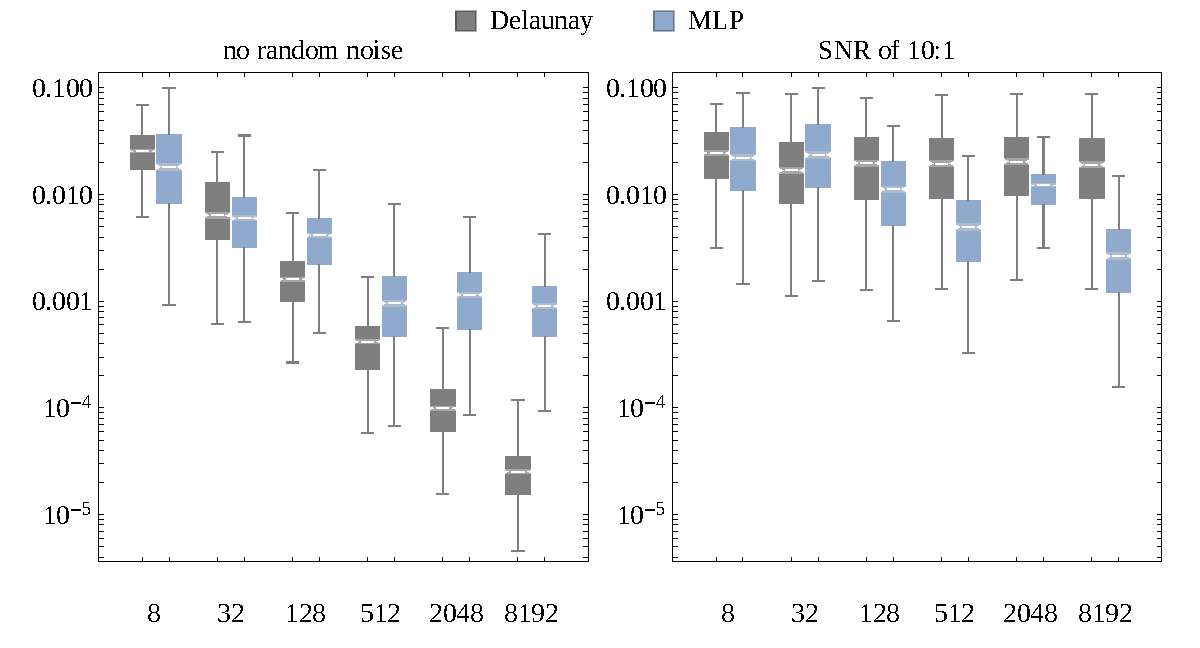
\includegraphics[width=0.9\textwidth,]{Fig2.pdf}};
    \node[below=of img, node distance=1cm, yshift=1cm] {Number of Data Points};
    \node[left=of img, node distance=0cm, rotate=90, anchor=center,yshift=-0.7cm] {Absolute Error};
  \end{tikzpicture}
  \caption{Delaunay and MLP approximations are constructed from Fekete
    points over the unit cube evaluating the test function $f(x) =
    \cos(\|x\|_2)$ for $x \in \mathbb{R}^2$. The figure shows the
    first/third quartiles at the box bottom/top, the second quartile
    (median) at the white bar, median 95\% confidence interval (cones,
    barely visible in figure), and whiskers at 3/2 of the adjacent
    interquartile ranges, for the absolute prediction error for each
    model at $1000$ random evaluation points. The left plot observes a
    perfect interpolation problem with exact evaluations of $f.$ The
    right plot observes a regression problem with uniform random noise
    giving values in $[.9 f(x),\ 1.1f(x)]$ for each $x.$ Both axes are
    log scaled.}
  \label{fig:convergence-2d}
\end{figure}

%% ===================================================================
\vspace{-2mm}
\subsection{Demonstration on an Analytic Test Function}
\label{sec:analytic}

The theoretical results constructed in Section \ref{sec:theory} for
(piecewise) linear interpolation are promising and apply directly to
Delaunay interpolation, however they are difficult to interpret in
context with approximation algorithms that do not have similar known
uniform error bounds. For that reason, an analytic function is used to
measure the error of a piecewise linear interpolant (Delaunay) and a
piecewise linear regressor (the MLP) when provided an increasing
amount of data with varying levels of random noise.

The test function chosen here for analysis resembles the
\textit{oscillatory} function used by \cite{barthelmann2000high}.
However, a slight modification is made to remove the simple dot
product structure (which is favorable for the MLP). Let $f(x)
=\cos(\|x\|_2)$ for $x \in \mathbb{R}^d$ where $d$ is either $2$
(Fig. \ref{fig:convergence-2d}) or $20$
(Fig. \ref{fig:convergence-20d}). This function has a bounded change
in gradient $2$-norm and hence meets the necessary Lipschitz condition
for the error bound. Data points and approximation points for this
test will be within the unit cube $[0,1]^d$.

The error of a linear interpolant constructed from well spaced points
is dominated by the distance to the nearest data point. In order to
uniformly decrease the distance to the nearest data point across the
unit cube, exponentially more data points must be available for
approximation. For this experiment $N = 2(4^i),$ $i = 1,$ $\ldots,$
$6,$ chosen points are kept well spaced by computing approximate
Fekete points. Fekete points have a history in potential theory
\cite{kovari_pommerenke_1968} and are most generally defined as those
points that maximize the absolute value of a Vandermonde
determinant. Here, the QR method outlined in \cite{bos2010computing}
is used to identify approximate Fekete points from a Vandermonde
matrix. A multivariate polynomial basis of size $2N$ is constructed
containing all polynomials of degree $\leq n$ for the largest $n$ such
that ${d+n \choose n} \leq 2N$ and $2N - {d+n \choose n}$
arbitrarily selected polynomials of degree $n + 1.$ The Vandermonde
matrix for these $2N$ polynomials is used to select $N$ approximate
Fekete points.

Finally an additional aspect is added to this test problem by
incorporating random uniform noise into the evaluations of $f.$ For
each test two experiments are executed, one with exact function
evaluations (for interpolation) and one with a constant signal-to-noise
(SNR) ratio of 10:1 (for regression).

\begin{figure}
  \centering
  \begin{tikzpicture}
    \node (img)  {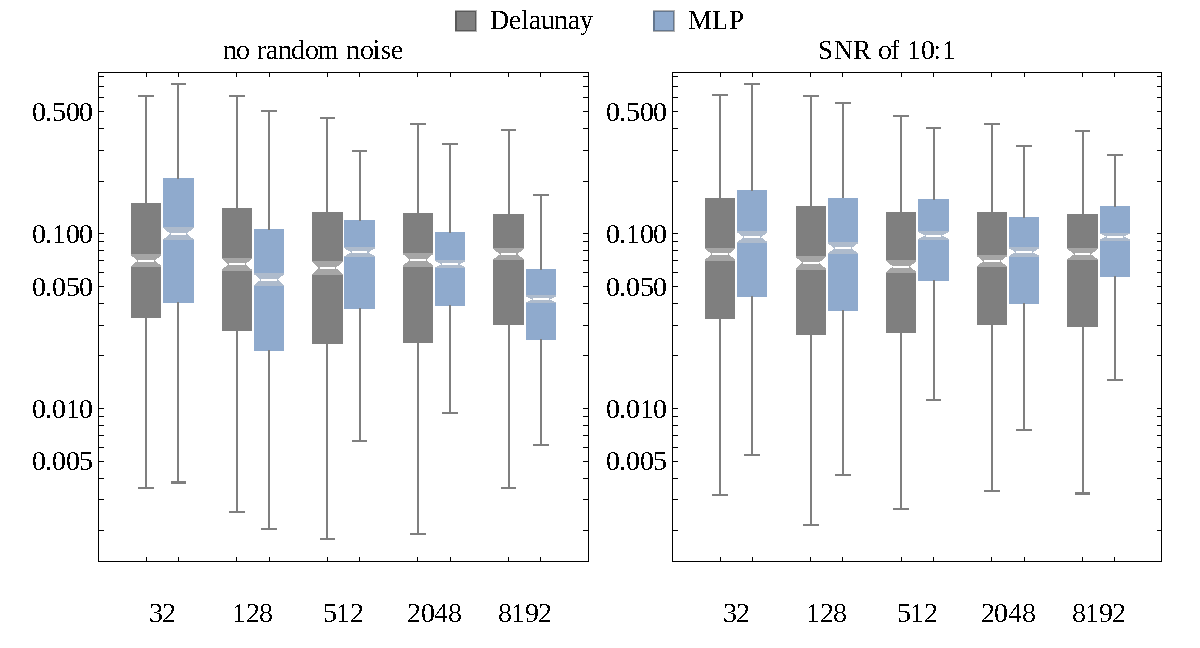
\includegraphics[width=0.9\textwidth,]{Fig3.pdf}};
    \node[below=of img, node distance=1cm, yshift=1cm] {Number of Data Points};
    \node[left=of img, node distance=0cm, rotate=90, anchor=center,yshift=-0.7cm] {Absolute Error};
  \end{tikzpicture}
  \caption{Delaunay and MLP approximations are constructed from Fekete
    points over the unit cube evaluating the test function $f(x) =
    \cos(\|x\|_2)$ for $x \in \mathbb{R}^{20}$. The details are the
    same as for Fig. \ref{fig:convergence-2d}.}
  \label{fig:convergence-20d}
\end{figure}


The bound from the theorem suggests that exponentially increasing the
number of data points should result in a decreasing error. The $d = 2$
test seen on the left half of Figure \ref{fig:convergence-2d} shows a
consistent decrease in error for Delaunay and also shows the eventual
accuracy plateau obtained by a parametric regression form (the MLP, at
roughly 500 points). On the right hand side of Figure
\ref{fig:convergence-2d} the random noise clearly prohibits Delaunay
from converging to $f$, while the MLP is able to improve its
approximation with more data points on average.  The convergence
result for a very low-dimensional problem like this is expected.
However, intuition fails for higher dimensional problems.

Figure \ref{fig:convergence-20d} shows the test function with $d = 20$
presents a significantly more challenging approximation problem than
its counterpart in low dimension. The same increase in number of data
points from 32 to 8192 causes no apparent improvement in approximation
for either the noise-free or the noisy problems. Perhaps unexpectedly,
the interpolation technique performs better than the regression
technique on the noisy data (right) in Figure
\ref{fig:convergence-20d}, and worse than the regression technique on
the noise-free data (left). This result emphasizes the relevance of
interpolation for problems in high dimension. It also reveals that the
outcome of MLP regressions can get worse when adding more data points.

In summary, the regime of interpolation is much greater for moderate
to high dimensional problems, even for functions with random noise
incorporated into their evaluation. Acknowledging the viability of
interpolation for problems of moderate dimension, the next section
will consider real-world problems of similar proportion (thousands of
examples in tens of dimensions).


%% ===================================================================
\vspace{-2mm}
\section{Data and Empirical Analysis}
\label{sec:data}

This section extends the comparison of interpolation and regression
algorithms to a sample of real-world problems. Five different data
sets of varying dimension and application are utilized to construct
approximations and compare the accuracy of different techniques.

In the following five subsections the sources and targets of each test
data set are described, as well as challenges and limitations related
to approximating these data. The distribution of response values being
modeled is presented followed by the distribution of approximation
errors for each algorithm. The plots for all five data sets have the
same format.

All five data sets are rescaled such that the domain of approximation
is the unit hypercube. The range of the first four data sets is the
real numbers, while the range of the fifth data set is the space of
cumulative distribution functions. All approximation techniques are
applied to the first four data sets, while only those interpolants
whose approximations are convex combinations of observed data are
applied to the final data set.

All approximations are constructed using $k$-fold cross validation as
described in \cite{kohavi1995study} with $k=10$. This approach
randomly partitions data into $k$ (nearly) equal sized sets. Each
algorithm is then evaluated by constructing an approximation over each
unique union of $k-1$ elements of the partition, making predictions
for points in the remaining element. As a result, each observed data
point is used in the construction of $k-1$ different approximations
and is approximated exactly once. The $k$-fold cross validation method
is data-efficient and provides an unbiased estimate of the expected
prediction error \cite{kohavi1995study}, however it should be noted
that neither this method nor others can provide a universally unbiased
estimator for the variance of prediction error \cite{bengio2004no}.

In addition to the figures displaying approximation results for each
data set, tables of accompanying numerical results are located in the
Appendix (Section \ref{sec:appendix}). All of the test data sets
capture underlying functions that are almost certainly stochastic. As
described in Section \ref{sec:introduction}, regression techniques
appear most appropriate for these problems. However, typically data
grows exponentially more sparse with increasing dimension. Given that
sparse data regressors tend towards interpolation and, as demonstrated
in Section \ref{sec:analytic}, interpolants produce similar (if not
identical) results, it is presumed that interpolants are equally
viable approximation techniques on these problems.

%% -------------------------------------------------------------------
\subsection{Forest Fire ($n = 504$, $d = 12$)}

\begin{figure}
  \centering
  \begin{tikzpicture}
    \node (img)  {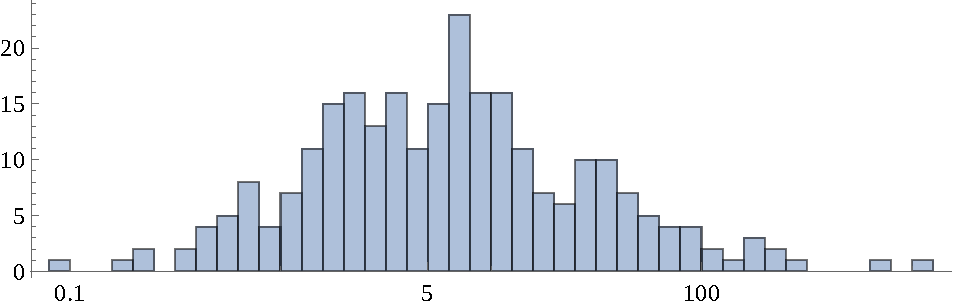
\includegraphics[width=0.75\textwidth,]{Fig4.pdf}};
    \node[below=of img, node distance=1cm, yshift=1cm] {Forest Fire Area Burned};
    \node[left=of img, node distance=0cm, rotate=90, anchor=center,yshift=-0.7cm] {Count};
  \end{tikzpicture}
  \caption{Histogram of forest fire area burned under recorded weather
    conditions. The data is presented on a $\ln$ scale because
    most values are small with exponentially fewer fires on record
    that burn large areas.}
  \label{fig:hist-forest-fire}
\end{figure}

\begin{figure}
  \centering
  \begin{tikzpicture}
    \node (img)  {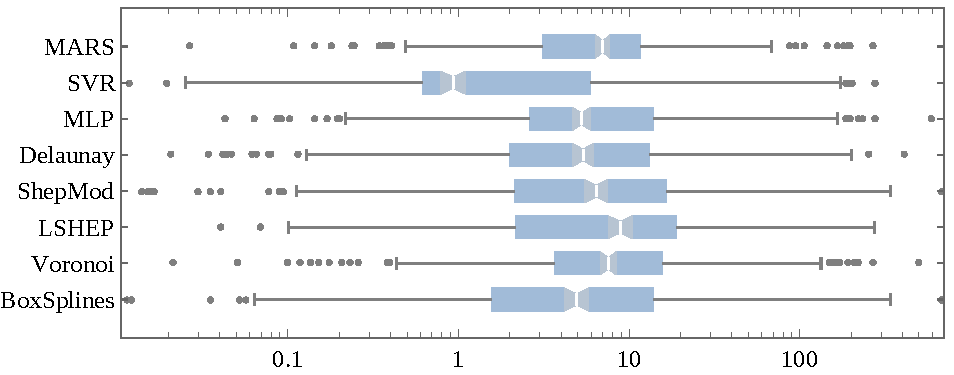
\includegraphics[width=0.8\textwidth,]{Fig5.pdf}};
    \node[below=of img, node distance=1cm, yshift=1cm] {Area Burned Error};
  \end{tikzpicture}
  \caption{All models are applied to approximate the amount of area
    that would be burned given environment conditions. $10$-fold cross
    validation as described in the beginning of Section \ref{sec:data}
    is used to evaluated each algorithm. This results in exactly one
    prediction from each algorithm for each data point. These boxes
    depict the median (middle bar), median $95\%$ confidence interval
    (cones), quartiles (box edges), fences at $3/2$ interquartile
    range (whiskers), and outliers (dots) of absolute prediction error
    for each model. Similar to Figure \ref{fig:hist-forest-fire}, the
    errors are presented on a $\ln$ scale. The numerical data
    corresponding to this figure is provided in Table
    \ref{table:error-forest-fire} in the Appendix.}
  \label{fig:error-forest-fire}
\end{figure}


The forest fire data set \cite{cortez2007data} describes the area of
Montesinho park burned over months of the year along with
environmental conditions. The twelve dimensions being used to model
burn area are the $x$ and $y$ spatial coordinates of burns in the
park, month of year (mapped to $x$, $y$ coordinates on a unit circle),
the FFMC, DMC, DC, and ISI indices (see source for details), the
temperature, relative humidity, wind speed, and outdoor rain. The
original analysis of this data set demonstrated it to be difficult to
model, likely due to the skew in response values.

As suggested by Figure \ref{fig:error-forest-fire}, the SVR has the
lowest absolute prediction errors for $80\%$ of the data, with MLP and
Delaunay being the nearest overall competitors. The effectiveness of
SVR on this data suggests the underlying function can be defined by
relatively few parameters, as well as the importance of capturing the
low-burn-area data points.
%% -------------------------------------------------------------------



%% -------------------------------------------------------------------
\subsection{Parkinson's Telemonitoring ($n = 5875$, $d = 19$)}

\begin{figure}
  \centering
  \begin{tikzpicture}
    \node (img)  {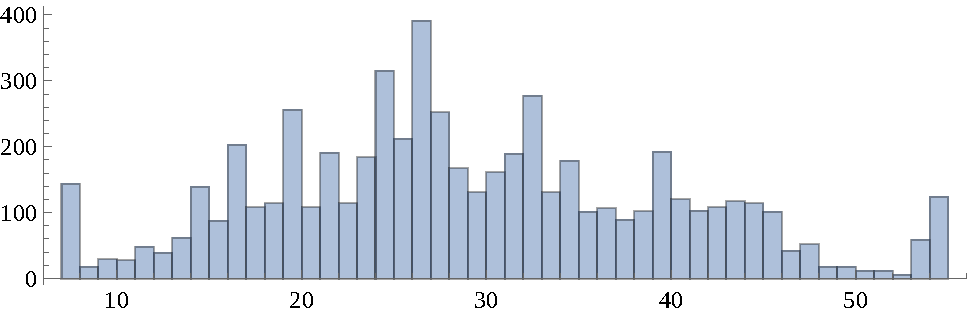
\includegraphics[width=0.75\textwidth,]{Fig6.pdf}};
    \node[below=of img, node distance=1cm, yshift=1cm] {Parkinson's Total UPDRS Score};
    \node[left=of img, node distance=0cm, rotate=90, anchor=center,yshift=-0.7cm] {Count};
  \end{tikzpicture}
  \caption{Histogram of the Parkinson's patient total UPDRS clinical
    scores that will be approximated by each algorithm.}
  \label{fig:hist-parkinsons}
\end{figure}

\begin{figure}
  \centering
  \begin{tikzpicture}
    \node (img)  {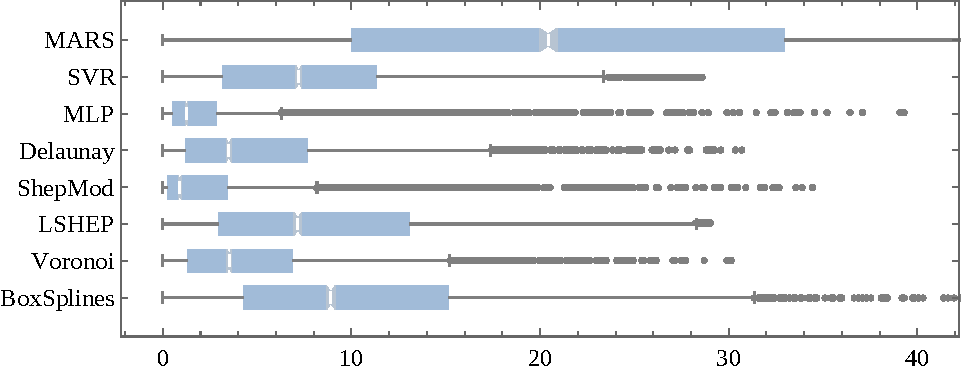
\includegraphics[width=0.8\textwidth,]{Fig7.pdf}};
    \node[below=of img, node distance=1cm, yshift=1cm] {Total UPDRS Score Error};
  \end{tikzpicture}
  \caption{All models are applied to approximate the total UPDRS score
    given audio features from patients' home life, using $10$-fold
    cross validation. These boxes depict the median (middle bar),
    median $95\%$ confidence interval (cones), quartiles (box edges),
    fences at $3/2$ interquartile range (whiskers), and outliers
    (dots) of absolute prediction error for each model. The numerical
    data corresponding to this figure is provided in Table
    \ref{table:error-parkinsons} in the Appendix.}
  \label{fig:error-parkinsons}
\end{figure}

The second data set for evaluation \cite{tsanas2010accurate} is
derived from a speech monitoring study with the intent to
automatically estimate Parkinson's disease symptom development in
Parkinson's patients. The function to be approximated is a
time-consuming clinical evaluation measure referred to as the UPDRS
score. The total UPDRS score given by a clinical evaluation is
estimated through 19 real numbers generated from biomedical voice
measures of in-home sound recordings.

Figure \ref{fig:error-parkinsons} shows the ShepMod algorithm has the
lowest minimum, first quartile, and median of absolute errors for this
problem, while providing the best prediction $66\%$ of the time. The
MLP has the lowest third quartile and provides the best prediction for
$32\%$ of approximations. The dominance of ShepMod may be due in part
to regular-interval total UPDRS scores provided by clinicians,
favoring a nearest-neighbor strategy of prediction.
%% -------------------------------------------------------------------



%% -------------------------------------------------------------------
\subsection{Australian Daily Rainfall Volume ($n = 2609$, $d = 23$)}

\begin{figure}
  \centering
  \begin{tikzpicture}
    \node (img)  {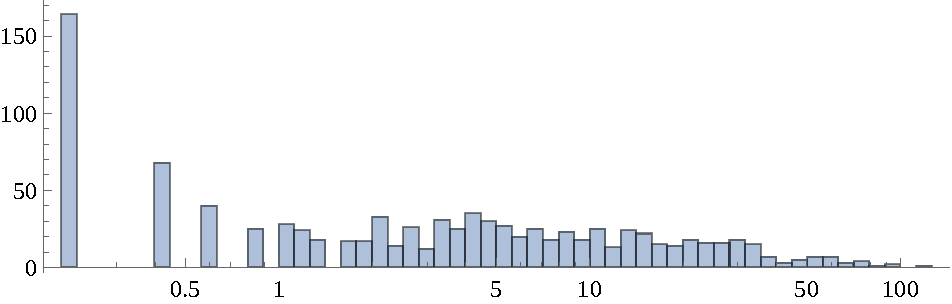
\includegraphics[width=0.75\textwidth,]{Fig8.pdf}};
    \node[below=of img, node distance=1cm, yshift=1cm] {Daily Rainfall in Sydney};
    \node[left=of img, node distance=0cm, rotate=90, anchor=center,yshift=-0.7cm] {Count};
  \end{tikzpicture}
  \caption{Histogram of daily rainfall in Sydney, Australia, presented
    on a $\ln$ scale because the frequency of larger amounts of
    rainfall is significantly less. There is a peak in occurrence of
    the value $0$, which has a notable effect on the resulting model
    performance.}
  \label{fig:hist-weather}
\end{figure}

\begin{figure}
  \centering
  \begin{tikzpicture}
    \node (img)  {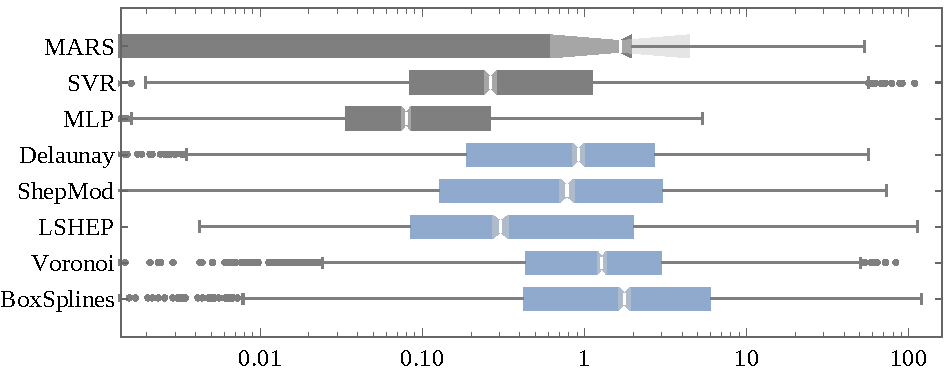
\includegraphics[width=0.8\textwidth,]{Fig9.pdf}};
    \node[below=of img, node distance=1cm, yshift=1cm] {Sydney Rainfall Tomorrow Error};
  \end{tikzpicture}
  \caption{All models are applied to approximate the amount of
    rainfall expected on the next calendar day given various sources
    of local meteorological data, using $10$-fold cross validation.
    These boxes depict the median (middle bar), median $95\%$
    confidence interval (cones), quartiles (box edges), fences at
    $3/2$ interquartile range (whiskers), and outliers (dots) of
    absolute prediction error for each model. The errors are presented
    on a $\ln$ scale, mimicking the presentation in Figure
    \ref{fig:hist-weather}. The numerical data corresponding to this
    figure is provided in Table \ref{table:error-weather} in the
    Appendix.}
  \label{fig:error-weather}
\end{figure}

The third data set for the total daily rainfall in Sydney, Australia
\cite{williams2009rattle} provides a slightly higher dimensional
challenge for the interpolants and regressors. This data is composed
of many meteorological readings from the region in a day including:
min and max temperatures, sunshine, wind speed directions (converted
to coordinates on a circle), wind speeds, and humidities throughout
the day, day of the year (converted to coordinates on a circle), and
the model must predict the amount of rainfall tomorrow.

While Figure \ref{fig:hist-weather} makes MARS look far better than
other techniques, it only provides the best prediction for $11\%$ of
points. The MLP has the lowest absolute error for $56\%$ of points and
LSHEP is best for $28\%$. MARS likely achieves such a low first
quartile due to the high occurrence of the value zero in the data.
%% -------------------------------------------------------------------



%% -------------------------------------------------------------------
\subsection{Credit Card Transaction Amount ($n = 5562$, $d = 28$)}

\begin{figure}
  \centering
  \begin{tikzpicture}
    \node (img)  {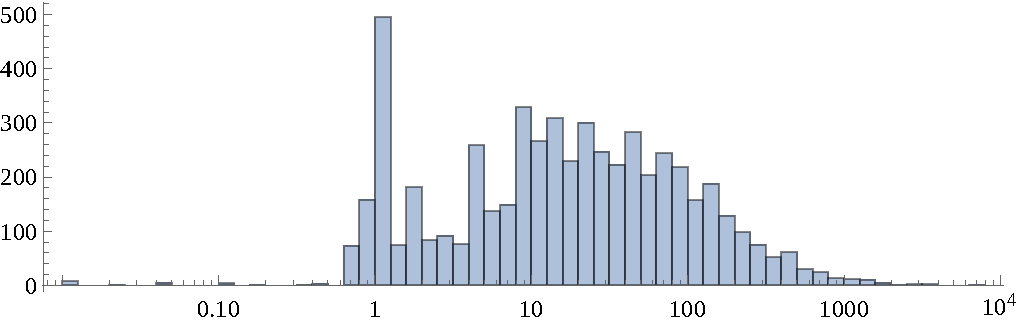
\includegraphics[width=0.75\textwidth,]{Fig10.pdf}};
    \node[below=of img, node distance=1cm, yshift=1cm] {Credit Card Transaction Amount};
    \node[left=of img, node distance=0cm, rotate=90, anchor=center,yshift=-0.7cm] {Count};
  \end{tikzpicture}
  \caption{Histogram of credit card transaction amounts, presented on
    a $\ln$ scale. The data contains a notable frequency peak around
    $\$1$ transactions. Fewer large purchases are made, but some large
    purchases are in excess of five orders of magnitude greater than
    the smallest purchases.}
  \label{fig:hist-credit-card}
\end{figure}

\begin{figure}
  \centering
  \begin{tikzpicture}
    \node (img)  {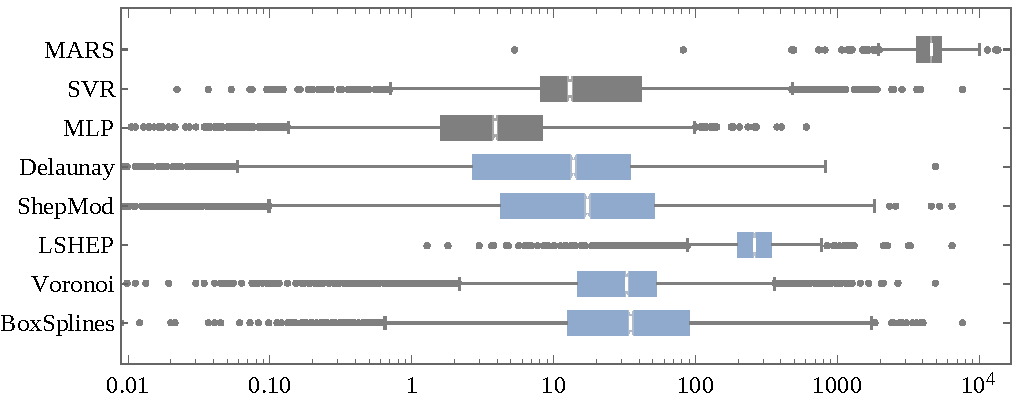
\includegraphics[width=0.8\textwidth,]{Fig11.pdf}};
    \node[below=of img, node distance=1cm, yshift=1cm] {Transaction Amount Error};
  \end{tikzpicture}
  \caption{All models are applied to approximate the expected
    transaction amount given transformed (and obfuscated) vendor and
    customer-descriptive features, using $10$-fold cross validation.
    These boxes depict the median (middle bar), median $95\%$
    confidence interval (cones), quartiles (box edges), fences at
    $3/2$ interquartile range (whiskers), and outliers (dots) of
    absolute prediction error for each model. The absolute errors in
    transaction amount predictions are presented on a $\ln$ scale,
    just as in Figure \ref{fig:hist-credit-card}. The numerical data
    corresponding to this figure is provided in Table
    \ref{table:error-credit-card} in the Appendix.}
  \label{fig:error-credit-card}
\end{figure}

The fourth test data set, and the final with a real-valued range, is a
collection of credit card transactions
\cite{pozzolo2015calibrating}. The provided data carries no direct
real-world meaning, being the output of a principle component analysis
on the original hidden source data. This obfuscation is done to
protect the information of the credit card users. This data has the
largest dimension of all considered, at 28. A model for this data
predicts the transaction amount given the vector of principle
component information.

As can be seen in Figure \ref{fig:error-credit-card}, the MLP
outperforms all other algorithms at the first, second, third, and
fourth quartiles. The MLP produces the lowest absolute error
prediction for $80\%$ of transactions, Delaunay bests the remaining
$20\%$. It is likely that with less data, Delaunay would be the best
performer.
%% -------------------------------------------------------------------


%% -------------------------------------------------------------------
\subsection{High Performance Computing I/O ($n = 3016$, $d = 4$)}

\begin{figure}
  \centering
  \begin{tikzpicture}
    \node (img)  {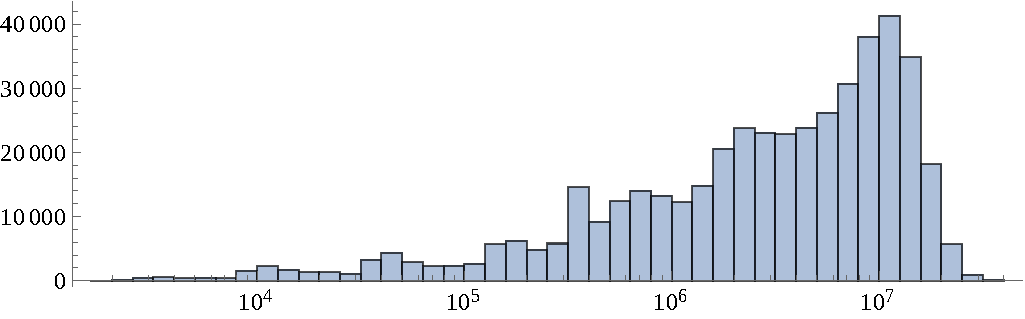
\includegraphics[width=0.75\textwidth,]{Fig12.pdf}};
    \node[below=of img, node distance=1cm, yshift=1cm] {I/O Read Throughput};
    \node[left=of img, node distance=0cm, rotate=90, anchor=center,yshift=-0.7cm] {Count};
  \end{tikzpicture}
  \caption{Histogram of the raw throughput values recorded during all
    IOzone tests across all system configurations. The distribution is
    skewed right, with few tests having significantly higher
    throughput than most others. The data is presented on a $\ln$
    scale.}
  \label{fig:hist-throughput}
\end{figure}

\begin{figure}
  \centering
  \begin{tikzpicture}
    \node (img)  {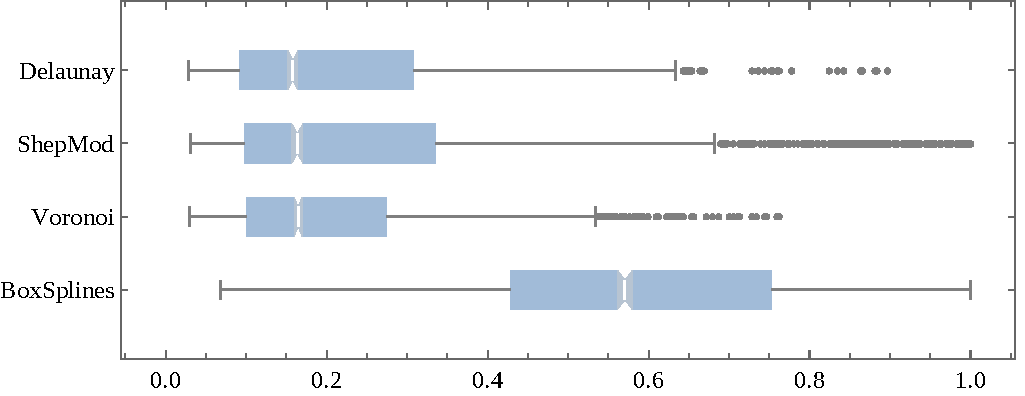
\includegraphics[width=0.8\textwidth,]{Fig13.pdf}};
    \node[below=of img, node distance=1cm, yshift=1cm] {Read Throughput KS Statistic};
  \end{tikzpicture}
  \caption{The models directly capable of predicting distributions are
    applied to predicting the expected CDF of I/O throughput at a
    previously unseen system configuration, using $10$-fold cross
    validation. The KS statistic (max norm) between the observed
    distribution at each system configuration and the predicted
    distribution is recorded and presented above. Note that the above
    figure is \textit{not} log-scaled like Figure
    \ref{fig:hist-throughput}. The numerical data corresponding to
    this figure is provided in Table \ref{table:error-throughput} in
    the Appendix.}
  \label{fig:error-throughput}
\end{figure}

The final of five data sets is derived from \cite{cameron2019moana},
which provides four-dimensional distribution data by executing the
IOzone benchmark \cite{iozone} on a computer system and varying the
system's file size, record size, thread count, and CPU frequency. At
each configuration, IOzone samples the I/O file-read throughput (in
bytes per second) 150 times. Empirical distribution function points
are computed from each set of 150 executions, which are interpolated
with a piecewise cubic Hermite interpolating polynomial
\cite{fritsch1980monotone} to approximate the CDF. All interpolation
algorithms with the exception of LSHEP are used to approximate these
CDFs from system configurations.

Delaunay achieves the lowest KS statistic (max norm difference) for
$62\%$ of approximations, while Voronoi is best for the remaining
$38\%$. Figure \ref{fig:error-throughput} shows that while Delaunay
may have more best predictions, the behavior of Voronoi may be
preferable.
%% -------------------------------------------------------------------


%% -------------------------------------------------------------------
\begin{figure}
  \centering
  \begin{tikzpicture}
    \node (img)  {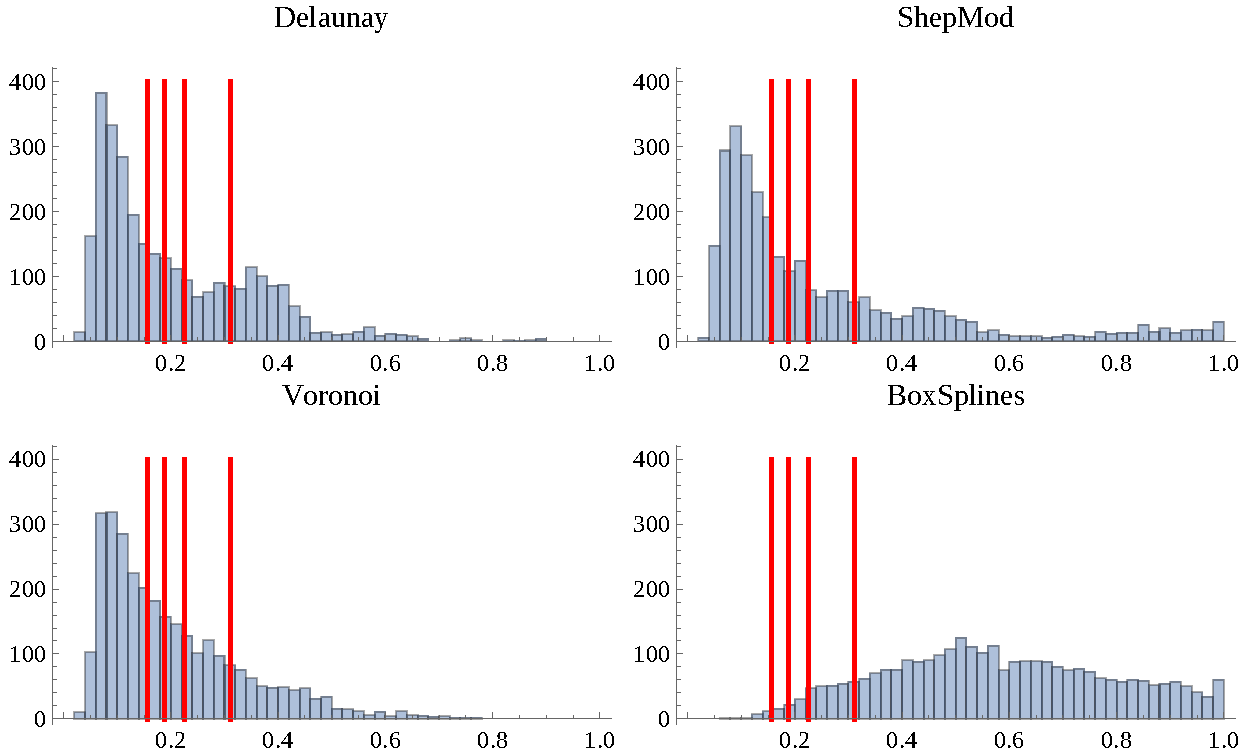
\includegraphics[width=0.8\textwidth]{Fig14.pdf}};
    \node[below=of img, node distance=1cm, yshift=1cm] {KS Statistic for Predicted vs. Actual};
    \node[left=of img, node distance=0cm, rotate=90, anchor=center,yshift=-0.7cm] {Count of KS Statistic};
  \end{tikzpicture}
  \caption{Histograms of the prediction error for each interpolant
    that produces predictions as convex combinations of observed data,
    using $10$-fold cross validation. The histograms show the KS
    statistics for the predicted throughput distribution versus the
    actual throughput distribution. The four vertical lines represent
    cutoff KS statistics given $150$ samples for commonly used
    $p$-values 0.05, 0.01, 0.001, $10^{-6}$, respectively. All
    predictions to the right of a vertical line represent CDF
    predictions that are significantly different (by respective
    $p$-value) from the actual distribution according to the KS
    test. The numerical counterpart to this figure is presented in
    Table \ref{table:null-hypothesis-results}.}
  \label{fig:throughput-prediction}
\end{figure}

\begin{table}
  \renewcommand{\arraystretch}{1.3}
  \centering
  \begin{tabular}{c|c|c|c|c}
               & $p = .05$         & $p = .01$         & $p = .001$        & $p = 10^{-6}$\\
    \hline
    Delaunay   & $\mathbf{50.3}\%$ & $\mathit{43.5}\%$ & $\mathit{36.2}\%$ & $\mathit{24.7}\%$\\
    ShepMod    & $\mathit{51.4}\%$ & $44.8\%$          & $38.1\%$          & $27.7\%$\\
    Voronoi    & $52.6\%$          & $\mathbf{43.4}\%$ & $\mathbf{34.4}\%$ & $\mathbf{19.1}\%$\\
    BoxSplines & $99.4\%$          & $98.5\%$          & $96.6\%$          & $89.3\%$\\
  \end{tabular}
  \caption{Numerical counterpart of the histogram data presented in
    Figure \ref{fig:throughput-prediction}. The columns display the
    percent of null hypothesis rejections by the KS-test when provided
    different selections of $p$-values for each algorithm. The
    algorithm with the lowest rejection rate at each $p$ is boldface,
    while the second lowest is italicized.}
  \label{table:null-hypothesis-results}
\end{table}


%% ===================================================================

Figure \ref{fig:throughput-prediction} expands on the KS statistic
results presented in Figure \ref{fig:error-throughput}. Agglomerate
errors for each algorithm resemble a Gamma distribution. The
percentages of significant prediction errors with varying $p$-values
are on display in Table \ref{table:null-hypothesis-results}. When
considering the $p=0.001$ results for each technique, a little over
one third of the predicted CDFs are significantly different from the
measured (and presumed) correct CDFs. However, it should be noted that
with 150 samples, the error of an empirical distribution function
(EDF) can reasonably be upwards of $.1$, which serves as a rough
estimate for the lower limit of achievable error. Globally, only a
third of Voronoi predictions fail to capture \textit{all} of the
characteristics of the CDFs at new system configurations.

\section{Discussion}
\label{sec:discussion}

                                                                      
\begin{table}
  \centering
  \begin{tabular}{c|r@{.}l|r@{.}l|r@{.}l}
    Algorithm & \multicolumn{2}{c|}{Avg. \% Best} & \multicolumn{2}{c|}{\multilinecell{Avg. Fit or \\ Prep. Time (s)}} & \multicolumn{2}{c}{Avg. App. Time (s)}\\
    \hline
    MARS        & \quad\quad$4$&$5$          & \quad\quad$20$&$0$s        & \qquad\quad $0$&$001$s\\
    SVR         & $\mathit{19}$&$\mathit{5}$ & $\mathbf{0}$&$\mathbf{5}$s & $\mathbf{0}$&$\mathbf{0001}$s\\
    MLP         & $\mathbf{43}$&$\mathbf{1}$ & $200$&$0$s                 & $0$&$001$s\\
    Delaunay    & $5$&$2$                    & $1$&$0$s                   & $1$&$0$s\\
    ShepMod     & $18$&$0$                   & $\textit{0}$&$\textit{7}$s & $\mathbf{0}$&$\mathbf{0001}$s\\
    LSHEP       & $8$&$4$                    & $2$&$0$s                   & $\mathbf{0}$&$\mathbf{0001}$s\\
    Voronoi     & $0$&$5$                    & $1$&$0$s                   & $0$&$04$s\\
    BoxSplines  & $3$&$5$                    & $0$&$8$s                   & $\mathit{0}$&$\mathit{0005}$s\\
  \end{tabular}
  \caption{This average of Appendix Tables
    \ref{table:best-forest-fire}, \ref{table:best-parkinsons},
    \ref{table:best-weather}, and \ref{table:best-credit-card}
    provides a gross summary of overall results. The columns display
    (weighted equally by data set, \textit{not} points) the average
    frequency with which any algorithm provided the lowest absolute
    error approximation, the average time to fit/prepare, and the
    average time required to approximate one point. The times have
    been rounded to one significant digit, as reasonably large
    fluctuations may be observed due to implementation hardware.
    Interpolants provide the lowest error approximation for nearly one
    third of all data, while regressors occupy the other two
    thirds. This result is obtained without any customized tuning or
    preprocessing to maximize the performance of any given
    algorithm. In practice, tuning and preprocessing may have large
    effects on approximation performance.}
  \label{table:avg-performance}
\end{table}

Table \ref{table:avg-performance} summarizes results across the four
test data sets with real-valued ranges. The interpolants discussed in
this paper produce the \textit{best} approximations roughly one third
of the time, and produce competitive approximations for almost all
data sets. These test problems are almost certainly
\textit{stochastic} in nature, but the high dimension leads to greater
data sparsity and model construction cost, making interpolation more
competitive.

The major advantages to interpolation lie in the near absence of
\textit{fit} time. Delaunay, LSHEP, and ShepMod all require pairwise
distance calculations, for numerical robustness (Delaunay) and to
determine the radii of influence for data points (LSHEP and
ShepMod). At least hundreds, and sometimes hundreds of thousands of
predictions can be made by the interpolants before the most widely
used regressor (MLP) finishes fitting these relatively small data
sets.  However, the computational complexities of all interpolants
presented are greater than linear in either dimension or number of
points, whereas the regressors' nonlinear complexity in dimension
generally comes from the model fitting optimization.

The new theoretical results presented in Section \ref{sec:theory}
directly apply to Delaunay interpolation, however the performance of
Delaunay does not appear significantly better than other algorithms on
these data sets.  This observation may be due to the stochastic nature
of the data, but it also speaks to the power of the approximations
generated by the different interpolation methods.  The strong
performance of other interpolants suggests that theoretical results
similar to those presented in this work can be achieved for the other
interpolants under reasonable assumptions.

Finally, most of the interpolants presented in this work benefit from
the ability to model \textit{any} function over real $d$-tuples with a
range that is closed under convex combinations. In general, error can
be quantified by any measure (particularly of interest may be
$L^2$, $L^\infty$, etc.). The results of the distribution prediction
case study indicate that interpolants can effectively predict
CDFs. The error analysis for that work relies on the KS statistic,
which captures the worst part of any prediction and hence provides a
conservatively large estimate of approximation error. The average
absolute errors in the predicted CDFs are always lower than the KS
statistics. However, the KS statistic was chosen as a metric because
of the important surrounding statistical theory. A nonnegligible
volume of predictions provide impressively low levels of average
absolute error in that final case study.



\section{Conclusion}
\label{sec:conclusion}

The major contributions of this work are: 1) new uniform theoretical
error bounds for piecewise linear interpolation in arbitrary dimension
(Section \ref{sec:theory}); 2) an empirical evaluation across
real-world problems that demonstrates interpolants produce
competitively accurate models of multivariate phenomenon when compared
with common regressors for sparse, moderately high dimensional
problems (Section \ref{sec:data}); and 3) a demonstration that some
interpolants generalize to interpolation in function spaces (Section
\ref{sec:error}), preserving monotonicity (with CDFs, e.g.), neither
of which common regressors can do.

The various interpolants discussed in this paper have been
demonstrated to effectively approximate multivariate phenomena up to
$30$ dimensions. The underlying constructions are theoretically
straightforward, interpretable, and yield reasonably accurate
predictions. Most of the interpolants' computational complexities make
them particularly suitable for applications in even higher
dimension. The major benefits of interpolation are seen when only a
small number of approximations ($\leq 1000$) are made from data and
when there are relatively few data points for the dimension (for
empirical results presented, $\log_d n \leq 5$). These findings
encourage broader application of interpolants to multivariate
approximation in science.

%\begin{acknowledgements}
%If you'd like to thank anyone, place your comments here
%and remove the percent signs.
%\end{acknowledgements}

%%====================================================================
%%====================================================================

\bibliographystyle{spmpsci}      % mathematics and physical sciences
\bibliography{paper}

\newpage

\begin{appendix}
\section{Appendix}
\label{sec:appendix}

\begin{normalsize}
\textbf{Statistical Terminology.} A random variable $X$ is precisely
defined by its \textit{cumulative distribution function} (CDF) $F_X$
and the derivative of the CDF, the \textit{probability density
  function} (PDF) $f_X.$ For any possible value $x$ of $X$, the
\textit{percentile} of $x$ is $100$ $F_X(x)$, the percentage values
drawn from $X$ that would be less than or equal to $x$ as the number
of samples tends towards infinity. The \textit{quartiles} of $X$ are
its $25$-th, $50$-th (median), and $75$-th percentiles. The absolute
difference between the median and an adjacent quartile is an
\textit{interquartile range}. Given an independent and identically
distributed sample from $X$ and presuming that $X$ has finite mean and
variance, a \textit{confidence interval} can be drawn about any
percentile estimated from the sample. A \textit{confidence interval}
describes the probability that a value lies within an interval. The
\textit{null hypothesis} is a statement (derived from some test
statistic) that the expected value of the observed statistic is equal
to an assumed population statistic. The $p$ value is the probability
of observing a given statistic if the \textit{null hypothesis} is
true.

\vspace{4mm}
\noindent \textbf{Raw Numerical Results.} The tables that follow show the
precise experimental results for all data sets presented in Section
\ref{sec:data}. The tests were all run serially on an otherwise idle
machine with a CentOS 6.10 operating system and an Intel i7-3770 CPU
operating at 3.4 GHz. The detailed performance results in the tables
that follow are very much dependent on the problem and the algorithm
implementation (e.g., some codes are TOMS software, some industry
distributions, and others are from conference paper venues). Different
typeface is used to show best performers, however not much
significance should be attached to ranking algorithms based on small
time (millisecond) differences. The results serve as a demonstration
of conceptual validity.

\end{normalsize}

\newpage

\vspace*{\fill}

\begin{table}[H]
  \centering
  \begin{tabular}{c|r@{.}l|r@{.}l|r@{.}l|r@{.}l|r@{.}l}
    \hline
    Algorithm & \multicolumn{2}{c}{Min}       & \multicolumn{2}{c}{$25^{th}$} & \multicolumn{2}{c}{$50^{th}$} & \multicolumn{2}{c}{$75^{th}$} & \multicolumn{2}{c|}{Max}\\
    \hline
    MARS      & $0$&$00984$                   & $3$&$11$                      & $7$&$01$                      & $\mathit{11}$&$\mathit{7}$    & $1090$&$0$\\
    SVR       & $0$&$0118$                    & $\mathbf{0}$&$\mathbf{615}$   & $\mathbf{0}$&$\mathbf{931}$   & $\mathbf{5}$&$\mathbf{89}$    & $1090$&$0$\\
    MLP       & $0$&$0426$                    & $2$&$63$                      & $5$&$27$                      & $14$&$0$                      & $1090$&$0$\\
    Delaunay  & $\mathbf{0}$&$\mathbf{0}$     & $1$&$98$                      & $5$&$37$                      & $13$&$1$                      & $\mathit{1080}$&$\mathit{0}$\\
    ShepMod   & $\mathbf{0}$&$\mathbf{0}$     & $1$&$93$                      & $6$&$27$                      & $16$&$0$                      & $1090$&$0$\\
    LSHEP     & $0$&$04$                      & $2$&$17$                      & $8$&$87$                      & $19$&$1$                      & $\mathbf{1070}$&$\mathbf{0}$\\
    Voronoi   & $\mathit{0}$&$\mathit{00982}$ & $3$&$65$                      & $7$&$56$                      & $15$&$6$                      & $1090$&$0$\\
    BoxSpline & $\mathbf{0}$&$\mathbf{0}$     & $\mathit{1}$&$\mathit{27}$    & $\mathit{4}$&$\mathit{61}$    & $12$&$6$                      & $1090$&$0$\\
    \hline
  \end{tabular}
  \caption{This numerical data accompanies the visual provided in
    Figure \ref{fig:error-forest-fire}. The columns of absolute error
    percentiles correspond to the minimum, first quartile, median,
    third quartile, and maximum absolute errors respectively. The
    minimum of each column is boldface, while the second lowest value
    is italicized. All values are rounded to three significant
    digits.}
  \label{table:error-forest-fire}
\end{table}

\begin{table}[H]
  \centering
  \begin{tabular}{|c|r@{.}l| c |r@{.}l|r@{.}l|r@{.}l|}
    \cline{1-3}\cline{5-10}
    Algorithm & \multicolumn{2}{c|}{\% Best}   &  & \multicolumn{2}{c|}{Fit/Prep. Time (s)} & \multicolumn{2}{c|}{App. Time (s)} & \multicolumn{2}{c|}{Total App. Time (s)}\\
    \cline{1-3}\cline{5-10}
    MARS      & \quad$7$&$3$                   &  & \quad\quad$29$&$1$                      & \quad$0$&$00137$                   & \quad\quad\quad$0$&$0686$\\
    SVR       & $\mathbf{78}$&$\mathbf{0}$     &  & $\mathbf{0}$&$\mathbf{00584}$           & $\mathit{0}$&$\mathit{0000620}$    & $\mathit{0}$&$\mathit{00310}$\\
    MLP       & $0$&$0$                        &  & $32$&$8$                                & $0$&$000871$                       & $0$&$0436$\\
    Delaunay  & $0$&$2$                        &  & $0$&$0151$                              & $0$&$0234$                         & $1$&$18$\\
    ShepMod   & $2$&$0$                        &  & $\mathit{0}$&$\mathit{00634}$           & $0$&$0000644$                      & $0$&$00322$\\
    LSHEP     & $5$&$1$                        &  & $0$&$0275$                              & $\mathbf{0}$&$\mathbf{0000463}$    & $\mathbf{0}$&$\mathbf{00231}$\\
    Voronoi   & $0$&$0$                        &  & $0$&$0152$                              & $0$&$000396$                       & $0$&$0198$\\
    BoxSpline & $\mathit{9}$&$\mathit{7}$      &  & $0$&$00724$                             & $0$&$0000978$                      & $0$&$00489$\\
    \cline{1-3}\cline{5-10}
  \end{tabular}
  \caption{The left above shows how often each algorithm had the
    lowest absolute error approximating forest fire data in Table
    \ref{table:error-forest-fire}. On the right columns are median fit
    time of 454 points, median time for one approximation, and median
    time approximating 50 points.}
  \label{table:best-forest-fire}
\end{table}

\vspace*{\fill}
\newpage

\begin{table}
  \centering
  \begin{tabular}{c|r@{.}l|r@{.}l|r@{.}l|r@{.}l|r@{.}l}
    \hline
    Algorithm & \multicolumn{2}{c}{Min}                   & \multicolumn{2}{c}{$25^{th}$} & \multicolumn{2}{c}{$50^{th}$} & \multicolumn{2}{c}{$75^{th}$} & \multicolumn{2}{c|}{Max}\\
    \hline
    MARS      & $0$&$00948$                               & $9$&$98$                      & $20$&$4$                      & $32$&$9$                      & $863$&$0$\\
    SVR       & $0$&$00233$                               & $3$&$15$                      & $7$&$21$                      & $11$&$3$                      & $\mathbf{28}$&$\mathbf{6}$\\
    MLP       & $0$&$0000239$                             & $\mathit{0}$&$\mathit{533}$   & $\mathit{1}$&$\mathit{25}$    & $\mathbf{2}$&$\mathbf{84}$    & $39$&$3$\\
    Delaunay  & $\mathit{3}$&$\mathit{72 \times 10^{-12}}$ & $1$&$2$                       & $3$&$5$                       & $7$&$67$                      & $30$&$7$\\
    ShepMod   & $\mathbf{0}$&$\mathbf{0}$                 & $\mathbf{0}$&$\mathbf{255}$   & $\mathbf{0}$&$\mathbf{908}$   & $\mathit{3}$&$\mathit{43}$    & $34$&$5$\\
    LSHEP     & $0$&$00254$                               & $2$&$93$                      & $7$&$16$                      & $13$&$1$                      & $\mathit{29}$&$\mathit{0}$\\
    Voronoi   & $\mathbf{0}$&$\mathbf{0}$                 & $1$&$29$                      & $3$&$52$                      & $6$&$87$                      & $30$&$1$\\
    BoxSpline & $0$&$006$                                 & $4$&$3$                       & $8$&$91$                      & $15$&$1$                      & $45$&$3$\\
    \hline
  \end{tabular}
  \caption{This numerical data accompanies the visual provided in
    Figure \ref{fig:error-parkinsons}. The columns of absolute error
    percentiles correspond to the minimum, first quartile, median,
    third quartile, and maximum absolute errors respectively. The
    minimum of each column is boldface, while the second lowest value
    is italicized. All values are rounded to three significant
    digits.}
  \label{table:error-parkinsons}
\end{table}

\begin{table}
  \centering
  \begin{tabular}{|c|r@{.}l| c |r@{.}l|r@{.}l|r@{.}l|}
    \cline{1-3}\cline{5-10}
    Algorithm & \multicolumn{2}{c|}{\% Best} &  & \multicolumn{2}{c|}{Fit/Prep. Time (s)} & \multicolumn{2}{c|}{App. Time (s)} & \multicolumn{2}{c|}{Total App. Time (s)}\\
    \cline{1-3}\cline{5-10}
    MARS      & \quad\,$0$&$0$               &  & \quad\quad\quad$37$&$9$                 & \quad\,\,$0$&$00253$               & \quad\quad\quad\,\,$1$&$48$\\
    SVR       & $0$&$1$                      &  & $\mathbf{0}$&$\mathbf{859}$             & $\mathit{0}$&$\mathit{000181}$     & $\mathit{0}$&$\mathit{106}$\\
    MLP       & $\mathit{32}$&$\mathit{0}$   &  & $348$&$0$                               & $0$&$00111$                        & $0$&$653$\\
    Delaunay  & $0$&$0$                      &  & $2$&$47$                                & $1$&$22$                           & $720$&$0$\\
    ShepMod   & $\mathbf{66}$&$\mathbf{4}$   &  & $\mathit{1}$&$\mathit{13}$              & $0$&$000182$                       & $0$&$107$\\
    LSHEP     & $0$&$0$                      &  & $2$&$39$                                & $\mathbf{0}$&$\mathbf{000144}$     & $\mathbf{0}$&$\mathbf{0845}$\\
    Voronoi   & $1$&$6$                      &  & $2$&$77$                                & $0$&$0274$                         & $16$&$1$\\
    BoxSpline & $0$&$0$                      &  & $1$&$26$                                & $0$&$000643$                       & $0$&$377$\\
    \cline{1-3}\cline{5-10}
  \end{tabular}
  \caption{The left above shows how often each algorithm had the
    lowest absolute error approximating Parkinson's data in Table
    \ref{table:error-parkinsons}. On the right columns are median fit
    time of 5288 points, median time for one approximation, and median
    time approximating 587 points.}
  \label{table:best-parkinsons}
\end{table}


\begin{table}
  \centering
  \begin{tabular}{c|r@{.}l|r@{.}l|r@{.}l|r@{.}l|r@{.}l}
    \hline
    Algorithm & \multicolumn{2}{c}{Min}                    & \multicolumn{2}{c}{$25^{th}$}              & \multicolumn{2}{c}{$50^{th}$}  & \multicolumn{2}{c}{$75^{th}$}  & \multicolumn{2}{c|}{Max}\\
    \hline
    MARS      & $\mathit{6}$&$\mathit{45 \times 10^{-15}}$ & $\mathbf{2}$&$\mathbf{70 \times 10^{-14}}$ & $1$&$66$                       & $1$&$96$                       & $\mathit{53}$&$\mathit{3}$\\
    SVR       & $0$&$0000915$                              & $0$&$0833$                                 & $0$&$263$                      & $\mathit{1}$&$\mathit{13}$     & $109$&$0$\\
    MLP       & $0$&$0000689$                              & $0$&$0337$                                 & $\mathbf{0}$&$\mathbf{0795}$   & $\mathbf{0}$&$\mathbf{264}$    & $\mathbf{5}$&$\mathbf{31}$\\
    Delaunay  & $\mathbf{0}$&$\mathbf{0}$                  & $0$&$187$                                  & $0$&$919$                      & $2$&$72$                       & $56$&$3$\\
    ShepMod   & $\mathbf{0}$&$\mathbf{0}$                  & $0$&$0957$                                 & $0$&$685$                      & $2$&$9$                        & $73$&$2$\\
    LSHEP     & $\mathbf{0}$&$\mathbf{0}$                  & $\mathit{0}$&$\mathit{0153}$               & $\mathit{0}$&$\mathit{106}$    & $1$&$17$                       & $113$&$0$\\
    Voronoi   & $\mathbf{0}$&$\mathbf{0}$                  & $0$&$43$                                   & $1$&$28$                       & $2$&$94$                       & $83$&$8$\\
    BoxSpline & $\mathbf{0}$&$\mathbf{0}$                  & $0$&$342$                                  & $1$&$59$                       & $5$&$53$                       & $119$&$0$\\
    \hline
  \end{tabular}
  \caption{This numerical data accompanies the visual provided in
    Figure \ref{fig:error-weather}. The columns of absolute error
    percentiles correspond to the minimum, first quartile, median,
    third quartile, and maximum absolute errors respectively. The
    minimum value of each column is boldface, while the second lowest
    is italicized. All values are rounded to three significant
    digits.}
  \label{table:error-weather}
\end{table}

\begin{table}
  \centering
  \begin{tabular}{|c|r@{.}l| c |r@{.}l|r@{.}l|r@{.}l|}
    \cline{1-3}\cline{5-10}
    Algorithm & \multicolumn{2}{c|}{\% Best} &  & \multicolumn{2}{c|}{Fit/Prep. Time (s)}    & \multicolumn{2}{c|}{App. Time (s)} & \multicolumn{2}{c|}{Total App. Time (s)}\\
    \cline{1-3}\cline{5-10}
    MARS      & \,\,\,\,$10$&$7$             &  & \quad\quad\quad$\mathit{0}$&$\mathit{151}$ & \quad$0$&$000117$                  & \quad\quad\quad\,\,$0$&$0304$\\
    SVR       & $0$&$0$                      &  & $\mathbf{0}$&$\mathbf{133}$                & $\mathbf{0}$&$\mathbf{0000947}$    & $\mathbf{0}$&$\mathbf{0246}$\\
    MLP       & $\mathbf{60}$&$\mathbf{9}$   &  & $169$&$0$                                  & $0$&$00137$                        & $0$&$356$\\
    Delaunay  & $0$&$1$                      &  & $0$&$664$                                  & $0$&$886$                          & $230$&$0$\\
    ShepMod   & $3$&$5$                      &  & $0$&$265$                                  & $0$&$000128$                       & $0$&$0333$\\
    LSHEP     & $\mathit{28}$&$\mathit{4}$   &  & $0$&$874$                                  & $\mathit{0}$&$\mathit{0000975}$    & $\mathit{0}$&$\mathit{0254}$\\
    Voronoi   & $0$&$2$                      &  & $0$&$675$                                  & $0$&$0270$                         & $7$&$01$\\
    BoxSpline & $4$&$1$                      &  & $0$&$330$                                  & $0$&$000406$                       & $0$&$106$\\
    \cline{1-3}\cline{5-10}
  \end{tabular}
  \caption{Left table shows how often each algorithm had the lowest
    absolute error approximating Sydney rainfall data in Table
    \ref{table:error-weather}. On the right columns are median fit
    time of 2349 points, median time for one approximation, and median
    time approximating 260 points.}
  \label{table:best-weather}
\end{table}


\begin{table}
  \centering
  \begin{tabular}{c|r@{.}l|r@{.}l|r@{.}l|r@{.}l|r@{.}l}
    \hline
    Algorithm & \multicolumn{2}{c}{Min}                    & \multicolumn{2}{c}{$25^{th}$} & \multicolumn{2}{c}{$50^{th}$} & \multicolumn{2}{c}{$75^{th}$} & \multicolumn{2}{c|}{Max}\\
    \hline
    MARS      & $5$&$36$                                   & $3610$&$0$                    & $4580$&$0$                    & $5450$&$0$                    & $13400$&$0$\\
    SVR       & $0$&$00706$                                & $8$&$14$                      & $\mathit{13}$&$\mathit{0}$    & $41$&$6$                      & $7690$&$0$\\
    MLP       & $0$&$00151$                                & $\mathbf{1}$&$\mathbf{6}$     & $\mathbf{3}$&$\mathbf{86}$    & $\mathbf{8}$&$\mathbf{34}$    & $\mathbf{604}$&$\mathbf{0}$\\
    Delaunay  & $\mathbf{0}$&$\mathbf{0}$                  & $\mathit{2}$&$\mathit{69}$    & $13$&$8$                      & $\mathit{35}$&$\mathit{0}$    & $\mathit{4840}$&$\mathit{0}$\\
    ShepMod   & $\mathbf{0}$&$\mathbf{0}$                  & $4$&$21$                      & $17$&$3$                      & $51$&$6$                      & $6510$&$0$\\
    LSHEP     & $1$&$27$                                   & $199$&$0$                     & $260$&$0$                     & $343$&$0$                     & $6530$&$0$\\
    Voronoi   & $\mathit{2}$&$\mathit{89 \times 10^{-10}}$ & $14$&$7$                      & $32$&$8$                      & $52$&$9$                      & $4860$&$0$\\
    BoxSpline & $\mathbf{0}$&$\mathbf{0}$                  & $12$&$4$                      & $35$&$0$                      & $90$&$1$                      & $7690$&$0$\\
    \hline
  \end{tabular}
  \caption{This numerical data accompanies the visual provided in
    Figure \ref{fig:error-credit-card}. The columns of absolute error
    percentiles correspond to the minimum, first quartile, median,
    third quartile, and maximum absolute errors respectively. The
    minimum value of each column is boldface, while the second lowest
    is italicized. All values are rounded to three significant
    digits.}
  \label{table:error-credit-card}
\end{table}

\begin{table}
  \centering
  \begin{tabular}{|c|r@{.}l| c |r@{.}l|r@{.}l|r@{.}l|}
    \cline{1-3}\cline{5-10}
    Algorithm & \multicolumn{2}{c|}{\% Best} &  & \multicolumn{2}{c|}{Fit/Prep. Time (s)} & \multicolumn{2}{c|}{App. Time (s)} & \multicolumn{2}{c|}{Total App. Time (s)}\\
    \cline{1-3}\cline{5-10}
    MARS      & \quad\,$0$&$0$               &  & \quad\quad\quad$22$&$0$                 & \quad$0$&$00148$                   & \quad\quad\quad\,\,$0$&$820$\\
    SVR       & $0$&$0$                      &  & $\mathbf{1}$&$\mathbf{01}$              & $\mathit{0}$&$\mathit{000210}$     & $\mathit{0}$&$\mathit{117}$\\
    MLP       & $\mathbf{79}$&$\mathbf{5}$   &  & $290$&$0$                               & $0$&$000714$                       & $0$&$397$\\
    Delaunay  & $\mathit{20}$&$\mathit{5}$   &  & $3$&$12$                                & $3$&$71$                           & $2070$&$0$\\
    ShepMod   & $0$&$1$                      &  & $\mathit{1}$&$\mathit{4}5$              & $0$&$000220$                       & $0$&$122$\\
    LSHEP     & $0$&$0$                      &  & $3$&$47$                                & $\mathbf{0}$&$\mathbf{000176}$     & $\mathbf{0}$&$\mathbf{0981}$\\
    Voronoi   & $0$&$0$                      &  & $3$&$32$                                & $0$&$0950$                         & $52$&$8$\\
    BoxSpline & $0$&$0$                      &  & $1$&$66$                                & $0$&$000956$                       & $0$&$532$\\
    \cline{1-3}\cline{5-10}
  \end{tabular}
  \caption{The left above shows how often each algorithm had the
    lowest absolute error approximating credit card transaction data
    in Table \ref{table:error-credit-card}. On the right columns are
    median fit time of 5006 points, median time for one approximation,
    and median time approximating 556 points.}
  \label{table:best-credit-card}
\end{table}



\begin{table}
  \centering
  \begin{tabular}{c|r@{.}l|r@{.}l|r@{.}l|r@{.}l|r@{.}l}
    \hline
    Algorithm & \multicolumn{2}{c}{Min}      & \multicolumn{2}{c}{$25^{th}$} & \multicolumn{2}{c}{$50^{th}$} & \multicolumn{2}{c}{$75^{th}$} & \multicolumn{2}{c|}{Max}\\
    \hline
    Delaunay  & $\mathbf{0}$&$\mathbf{0287}$ & $\mathbf{0}$&$\mathbf{0914}$  & $\mathbf{0}$&$\mathbf{158}$   & $\mathit{0}$&$\mathit{308}$   & $\mathit{0}$&$\mathit{897}$\\
    ShepMod   & $0$&$0307$                   & $\mathit{0}$&$\mathit{0983}$  & $\mathit{0}$&$\mathit{164}$   & $0$&$335$                     & $1$&$0$\\
    Voronoi   & $\mathit{0}$&$\mathit{0303}$ & $0$&$1$                       & $0$&$165$                     & $\mathbf{0}$&$\mathbf{274}$   & $\mathbf{0}$&$\mathbf{762}$\\
    BoxSpline & $0$&$0679$                   & $0$&$429$                     & $0$&$571$                     & $0$&$752$                     & $1$&$0$\\
    \hline
  \end{tabular}
  \caption{This numerical data accompanies the visual provided in
    Figure \ref{fig:error-throughput}. The columns of absolute error
    percentiles correspond to the minimum, first quartile, median,
    third quartile, and maximum KS statistics respectively between
    truth and guess for models predicting the distribution of I/O
    throughput that will be observed at previously unseen system
    configurations. The minimum value of each column is boldface,
    while the second lowest is italicized. All values are rounded to
    three significant digits.}
  \label{table:error-throughput}
\end{table}

\begin{table}
  \centering
  \begin{tabular}{|c|r@{.}l| c |r@{.}l|r@{.}l|r@{.}l|}
    \cline{1-3}\cline{5-10}
    Algorithm & \multicolumn{2}{c|}{\% Best}   &  & \multicolumn{2}{c|}{Fit/Prep. Time (s)} & \multicolumn{2}{c|}{App. Time (s)} & \multicolumn{2}{c|}{Total App. Time (s)}\\
    \cline{1-3}\cline{5-10}
    Delaunay  & \,\,$\mathbf{62}$&$\mathbf{0}$ &  & \quad\quad\quad$0$&$344$                & \quad$0$&$00984$                   & \quad\quad\,\,$2$&$71$\\
    ShepMod   & $0$&$0$                        &  & $\mathbf{0}$&$\mathbf{0884}$            & $\mathbf{0}$&$\mathbf{000145}$     & $\mathbf{0}$&$\mathbf{0436}$\\
    Voronoi   & $\mathit{38}$&$\mathit{0}$     &  & $0$&$360$                               & $0$&$00253$                        & $0$&$762$\\
    BoxSpline & $0$&$0$                        &  & $\mathit{0}$&$\mathit{0972}$            & $\mathit{0}$&$\mathit{000210}$     & $\mathit{0}$&$\mathit{0633}$\\
    \cline{1-3}\cline{5-10}
  \end{tabular}
  \caption{The left above shows how often each algorithm had the
    lowest KS statistic on the I/O throughput distribution data in
    Table \ref{table:error-throughput}. On the right columns are
    median fit time of 2715 points, median time for one approximation,
    and median time approximating 301 points.}
  \label{table:best-throughput}
\end{table}


\end{appendix}

\end{document}
